\graphicspath{ {Figures/technology_stack/} }
\chapter{Τεχνολογίες}\label{ch:Development Stack}
\section{Back-End}
	\subsection{Cloud}
	\subsubsection{Ευκαιρίες και προκλήσεις στον τομέα υγείας}
	Πρόσφατες έρευνες έδειξαν ότι το 75\% των διευθυντών πληροφοριακών συστημάτων ανέφεραν ότι θα χρειαστεί να χρησιμοποιήσουν τις τεχνολογίες του υπολογιστικού νέφους στο άμεσο μέλλον \cite{danekCanadaCloud}\cite{cloudComputingIncrease}. Στον τομέα υγείας πολλοί οργανισμοί, διευθυντές και ειδικοί του χώρου πιστεύουν ότι η τεχνολογία του υπολογιστικού νέφους μπορεί να βελτιώσει σημαντικά τις παρεχόμενες υπηρεσίες υγείας, ενώ παράλληλα να μειώσει αισθητά τα λειτουργικά κόστη\cite{Dudley2010}\cite{Schweitzer2012}\cite{Blumenthal2009}\cite{Kabachinski2011}. Επιπλέον μια αναφορά από τον Ευρωπαϊκό Οργανισμό για την Ασφάλεια Δικτύων και Πληροφοριών (ΕΝΙΣΑ) προβλέπει ότι ο νέος αυτός τεχνολογικός τομέας θα λάβει τεράστιες επενδύσεις στο χώρο της υγείας\cite{bannermanCloud}. 

Παρακάτω στο \ref{tab:health_cloud_challenges_opportunities} βλέπουμε σε μορφή πίνακα μια σύνοψη των ευκαιριών αλλά και των προκλήσεων που παρουσιάζει η τεχνολογία του υπολογιστικού νέφους για το χώρο της υγείας.
	
\begin{table}[h]
	\begin{center}
	    \begin{tabular}{|l| p{\dimexpr 0.45\linewidth-2\tabcolsep} | p{\dimexpr 0.45\linewidth-2\tabcolsep} |}
	    \hline
	    \rowcolor{grayy}
	    \textbf{Τομέας} & \textbf{Ευκαιρείες} & \textbf{Προκλήσεις}
	    \\ \hline    
	    \multirow{3}{*}{Διοίκησης} & Χαμηλότερο κόστος υποδομών του IT & Έλειψη εμπιστοσύνης των προμηθευτών υγείας \\
	    & Διάθεση υπολογιστικών πόρων on demand & Οργανωτική αδράνεια \\
	    & Σταδιακή πληρωμή ανάλογως τις ανάγκες & Απώλεια άμέσου ελέγχου δεδομένων \\ \hline
	    \multirow{3}{*}{Τεχνολογίας} & Μείωση εργασιών συντήρησης του ΙΤ & Προβλήματα εξάντλησης πόρων \\
	    & Ευελξία και επεκτασιμότητα υποδομών IT & Απρόβλεπτη συμπεριφορά \\
	    & Οικολογική λύση & Απώλεια άμέσου ελέγχου δεδομένων  \\ \hline
	    \multirow{3}{*}{Ασφάλειας} & Περισσότεροι πόροι για προστασία δεδομένων & Κατάχρηση προνομίων \\
	    & Αντιγραφή των δεδομένων σε πολλαπλές τοποθεσίες & Ασφάλεια των φυσικών αποθηκευτικών μέσων \\
	    & Δυναμικά επεκτάσιμοι πόροι ασφάλεια που αυξάνει την ελαστικότητα & Προβλήματα διαχείρησης κλειδιών κρυπτογράφησης \\ \hline
	    \end{tabular}
	    \caption{Ευκαιρείες και Προκλήσεις cloud στον χώρο της υγείας}
	    \label{tab:health_cloud_challenges_opportunities}
	\end{center}
\end{table}	
	\subsubsection{Θεωρητικό υπόβαθρο υπολογιστικού νέφους}
	To cloud computing (υπολογιστικό νέφος) όπως ορίζεται από το NIST (Εθνικό Ινστιτούτο Προτύπων και Τεχνολογίας)  είναι μια τεχνολογία, η οποία επιτρέπει την πρόσβαση από παντού, παρέχει μετά από αίτημα πρόσβαση στο δίκτυο για την κοινή χρήση προσαρμοστικών υπολογιστικών πόρων (π.χ., δίκτυα, servers, συστήματα αποθήκευσης, εφαρμογές και υπηρεσίες), μπορεί να ξεκινήσει και να αναπτυχθεί γρήγορα με ελάχιστη διαχείριση και χωρίς καμία αλληλεπίδραση με τον φορέα παροχής υπηρεσιών. \cite{cloudComputing} Το cloud computing παρέχει στους χρήστες και στις επιχειρήσεις διάφορες δυνατότητες για την αποθήκευση και την επεξεργασία των δεδομένων τους σε τρίτα κέντρα δεδομένων. \cite{Haghighat2015}
	
	Το cloud computing ουσιαστικά στηρίζεται στην κατανομή των πόρων με στόχο την επίτευξη συνοχής και οικονομίας μέσω ενός δικτύου και την μεγιστοποίηση της απόδοσης τους. Οι πόροι του cloud δεν είναι μόνο διαμοιραζόμενοι από πολλούς χρήστες αλλά μπορούν και να ανακατανεμηθούν δυναμικά ανάλογα με την ζήτηση, γεγονός που μπορεί να χρησιμοποιηθεί όταν κατανέμονται στους διάφορους χρήστες.  Για παράδειγμα, μια cloud εγκατάσταση ηλεκτρονικών υπολογιστών οι οποία εξυπηρετεί Ευρωπαίους χρήστες στην διάρκεια των Ευρωπαϊκών εργάσιμων ωρών μπορεί να ανακατανείμει τους ίδιους πόρους για να εξυπηρετήσει χρήστες στην Βόρεια Αμερική κατά τις εργάσιμες ώρες της Βόρειας Αμερικής σε μία διαφορετική εφαρμογή. Αυτή η προσέγγιση βοηθά στην μεγιστοποίηση της χρήσης της υπολογιστικής ισχύος ενώ ταυτόχρονα μειώνεται το ολικό κόστος των φυσικών πόρων καθώς χρησιμοποιούμε λιγότερη ενέργεια, κλιματισμό κ.λ.π. για να διατηρείται το σύστημα.Με χρήση του cloud computing πολλοί χρήστες μπορούν να έχουν πρόσβαση σε έναν server και να ανακτούν και να ανανεώνουν τα δεδομένα τους χωρίς να αγοράζουν άδειες για όλες τις διαφορετικές εφαρμογές. \cite{Grossm2009}
	
	Οι πάροχοι cloud συνήθως χρησιμοποιούν μοντέλο κοστολόγησης "πλήρωσε όσο χρησιμοποιήσεις".  Παρουσιάζει σπουδαιότητα λοιπόν το γεγονός ότι οι "πελάτες" μπορούν να εξοικονομήσουν χρηματικούς πόρους στο πέρασμα του χρόνου, καθώς χρησιμοποιώντας τους πόρους στο cloud, πληρώνουν μόνο για τους πόρους που χρησιμοποιούν και όχι για την αγορά και συντήρηση άφθονων μηχανημάτων (π.χ. εξυπηρετητών). Η λύση λοιπόν του cloud computing λοιπόν αποτελεί μία ιδιαίτερα ελκυστική προοπτική για τους χρήστες στους οποίους η χρήση των πόρων ποικίλλει σημαντικά καθώς και σε αυτούς στους οποίους  η αγορά μηχανημάτων και το κόστος συντήρησης τους αποτελούν σημαντικό τμήμα του προϋπολογισμού. 

	Ένα πλήρες σύστημα υπολογιστικού νέφους αποτελείται από τα εξής βασικά συστατικά : 
	\begin{itemize}
	\item Πελάτες - υπολογιστές. Πρόκειται για τις συσκευές των τελικών χρηστών, μέσω των οποίων οι ``πελάτες" αποκτούν πρόσβαση στο υπολογιστικό νέφος. Χωρίζονται σε τρεις κατηγορίες: τις κινητές συσκευές (mobile devices) που επιτρέπουν στον χρήστη την απομακρυσμένη πρόσβαση μετά από επεξεργασία του κατανεμημένου διακομιστή, τους παχείς πελάτες (thick clients) που είναι οι σταθεροί υπολογιστές ή τα λάπτοπ τα οποία συνδέονται στο cloud με χρήση ενός φυλλομετρητή και τους λεπτούς πελάτες (thin clients ) που είναι υπολογιστές με μικρή υπολογιστική ισχύ και χωρίς σκληρούς δίσκους, που εμφανίζουν τα δεδομένα αφού τα επεξεργαστεί πρώτα ο διακομιστής.
	\item Κέντρο δεδομένων. Είναι το σύνολο των διακομιστών, όπου τρέχουν οι εφαρμογές. Στο κέντρο δεδομένων εμπίπτουν και οι εικονικοί διακομιστές (σε έναν υπολογιστή γίνεται εγκατάσταση ώστε να επιτρέπεται η ταυτόχρονη ύπαρξη πολλαπλών στιγμιοτύπων από εικονικούς διακομιστές).
	\item Κατανεμημένους διακομιστές. Οι διακομιστές αυτοί βρίσκονται σε διαφορετικές γεωγραφικές θέσεις, έτσι ώστε να εξασφαλίζεται μεγαλύτερη ευελιξία και υψηλότερη ασφάλεια στις παροχές που προσφέρει το cloud computing. Έτσι μπορούν να αντιμετωπιστούν αποτελεσματικά περιπτώσεις παραβίασης ασφάλειας ή ανάγκης επιπλέον αποθηκευτικού χώρου και υπολογιστικής δύναμης.
	\end{itemize}		
	
	Στο σχήμα \ref{fig:cloud},φαίνεται μία σχηματική αναπαράσταση του συστήματος cloud computing.
	
			\begin{figure}[h]
	    \centering
	    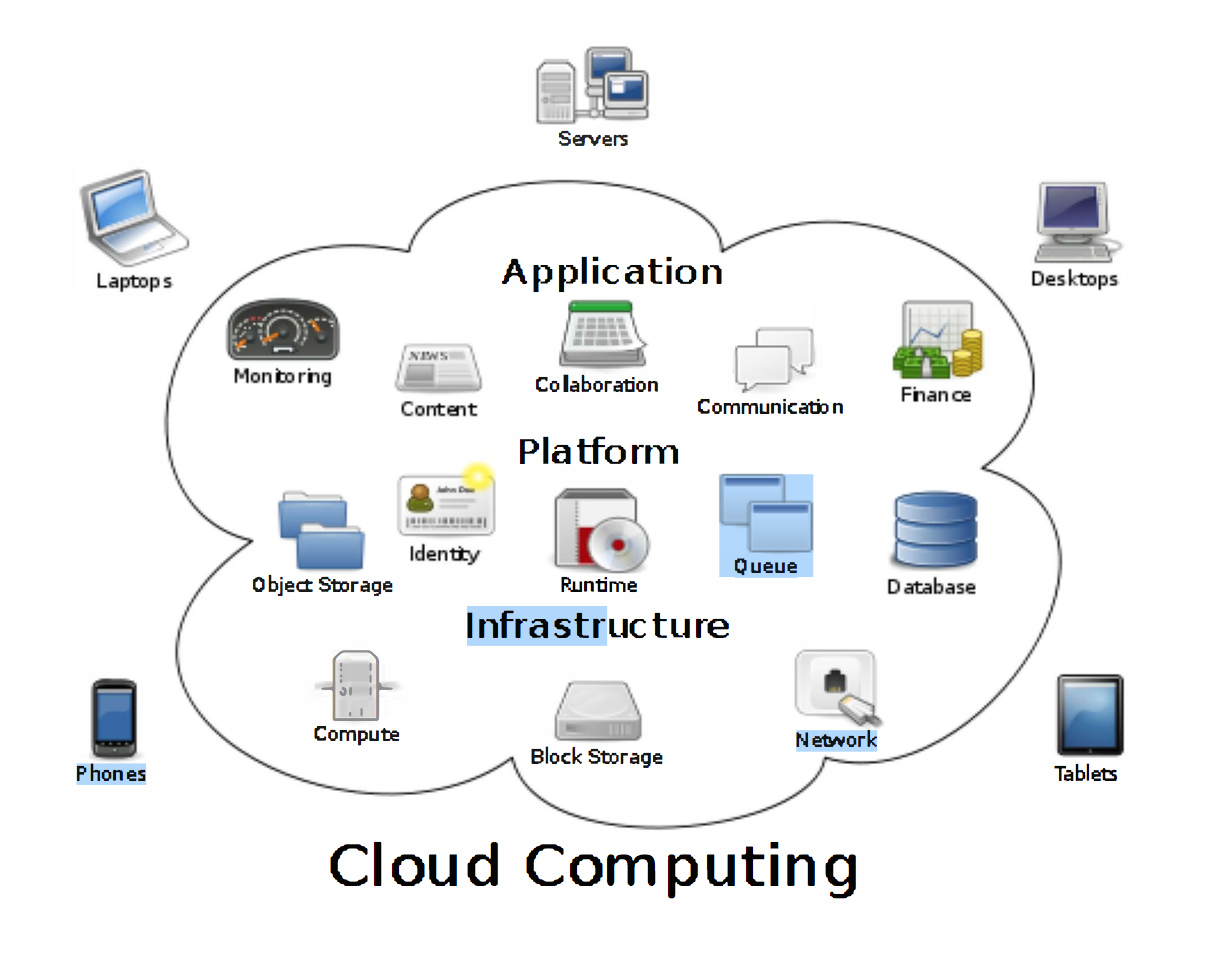
\includegraphics[width=0.7\textwidth]{cloud.png}
	    \caption{ Cloud Computing.  }
	    \label{fig:cloud}
	\end{figure}

		Το μοντέλο cloud αποτελείται από πέντε βασικά χαρακτηριστικά:
		\begin{itemize}
		\item Αυτοεξυπηρέτηση μετά από ζήτηση (On-demand self-service). Ο χρήστης των υπηρεσιών του νέφους μπορεί να χρησιμοποιεί τους υπολογιστικούς πόρους που χρειάζεται, όπως χρόνο στον server και αποθηκευτικό χώρο, αυτόματα και χωρίς να απαιτείται ανθρώπινη αλληλεπίδραση με τον φορέα παροχής υπηρεσιών. 
		\item Ευρεία πρόσβαση στο δίκτυο (Broad network access). Οι δυνατότητες που προσφέρονται είναι διαθέσιμες μέσω του δικτύου και προσβάσιμες μέσω τυποποιημένων μηχανισμών που προωθούν την χρήση ετερογενών πλατφορμών λεπτών ή παχέων πελατών (π.χ., κινητά τηλέφωνα, τάμπλετ, υπολογιστές). 
		\item Διάθεση των πόρων. Οι υπολογιστικοί πόροι των cloud παρόχων είναι συγκεντρωμένοι με χρήση ενός μοντέλου πολλαπλών ενοικιαστών (κάθε οργανισμός εργάζεται με ένα προσαρμοσμένο εικονικό στιγμιότυπο της εφαρμογής), έτσι ώστε να  μπορούν να ανατεθούν οι φυσικοί και εικονικοί πόροι ανάλογα με την ζήτηση των καταναλωτών. Οι παρεχόμενοι πόροι μπορεί να περιλαμβάνουν πόρους όπως μνήμη, επεξεργαστική ισχύ, εύρος δικτύου, εικονικές μηχανές.
		\item Μεγάλη ελαστικότητα (Rapid Elasticity). Οι δυνατότητες του cloud computing παρέχονται με μεγάλη ταχύτητα και προσαρμοστικότητα , ώστε να είναι σε θέση να κλιμακώνουν πολύ γρήγορα ανάλογα με την ζήτηση που υπάρχει και να φαίνονται απεριόριστες σε οποιαδήποτε ποσότητα και χρονική στιγμή ζητηθούν. 
		\item Μετρούμενη υπηρεσία (Measured Service). Τα cloud computing συστήματα πραγματοποιούν μετρήσεις, σε συγκεκριμένα επίπεδα αφαίρεσης ανάλογα με το είδος της υπηρεσίας (επεξεργασία, μνήμη, ενεργοί λογαριασμοί χρηστών). Με βάση αυτές τις μετρήσεις γίνεται έλεγχος και ενέργειες για τη βελτιστοποίηση της χρήσης των πόρων. Επιπλέον η χρήση των πόρων παρακολουθείται, ελέγχεται και καταγράφεται με αποτέλεσμα την παροχή διαφάνειας μεταξύ του χρήστη και του παρόχου του cloud.
		\end{itemize}	\cite{characteristicsCloud}\cite{nist}.

Το cloud computing μπορεί να διαχωριστεί με βάση τις υπηρεσίες που προσφέρει σε διάφορες κατηγορίες. Οι πιο βασικές, είναι α) η υποδομή ως μία υπηρεσία (IaaS), β) η πλατφόρμα ως μία υπηρεσία (PaaS) γ) το λογισμικό ως μία υπηρεσία (SaaS) και το δ) backend των κινητών σαν υπηρεσία(MBaaS), που είναι γνωστό σαν backend σαν υπηρεσία(BaaS).
\\*
		\subsubsection{IaaS}

		Η υποδομή σαν υπηρεσία προσφέρει πρόσβαση σε υπολογιστικούς πόρους στο εικονικό περιβάλλον του cloud, σε εικονικό υλικό (hardware). Το εικονικό υλικό περιλαμβάνει εικονικό χώρο server, συνδέσεις δικτύου, εύρος ζώνης, διευθύνσεις IP  και εξισορροπιστές φορτίου. Το σύνολο των πόρων του υλικού προκύπτει από ένα πλήθος servers και δικτύων που είναι κατανεμημένοι συνήθως σε διάφορα κέντρα δεδομένων και ο πάροχος cloud είναι υπεύθυνος για τη διατήρηση τους. Στον χρήστη δίνεται πρόσβαση στους πόρους του cloud ώστε να μπορεί να χτίσει τις δικές του πλατφόρμες πληροφορικής. 
		
		Οι IaaS υπηρεσίες μπορούν σε συνδυασμό με άλλες υπηρεσίες του cloud να χρησιμοποιηθούν για τη δημιουργία οικονομικά συμφέρουσων και εύκολα επεκτάσιμων λύσεων πληροφορικής, όπου οι δυσκολίες και τα έξοδα διαχείρισης έχουν ανατεθεί στον πάροχο cloud. Όταν οι δραστηριότητες του χρήστη κλιμακώνονται, και επιθυμεί μία επέκταση ή σμίκρυνση των υπολογιστικών πόρων, τότε μπορεί να αντλήσει ή να εγκαταλείψει πόρους cloud χωρίς να χρειάζεται να αγοραστεί, να εγκατασταθεί και να ενσωματωθεί νέο υλικό από τον ίδιο. \cite{IaasService}
		
		Η υπηρεσία IaaS προσφέρει επεκτασιμότητα. Οι πόροι είναι διαθέσιμοι την χρονική στιγμή που τους χρειάζεται ο πελάτης και έτσι αποφεύγονται καθυστερήσεις στην επέκταση της παραγωγικής ικανότητας. Επιπλέον, δεν υπάρχει η ανάγκη για επενδύσεις στο υλικό (hardware). Το "φυσικό" υλικό, το οποίο βρίσκεται πίσω από την IaaS υπηρεσία, έχει στηθεί και συντηρείται από τον πάροχο cloud, με αποτέλεσμα να εξοικονομείται χρόνος και χρήμα στην πλευρά του χρήστη.  Ένα βασικό πλεονέκτημα είναι ότι ο πελάτης κοστολογείται με βάση τη χρήση και πληρώνει μόνο τους πόρους που χρησιμοποιεί. Οι υπηρεσίες μπορούν να προσεγγισθούν από οποιαδήποτε τοποθεσία, αρκεί ο χρήστης να έχει πρόσβαση στο ίντερνετ και τα κατάλληλα διαπιστευτήρια, γεγονός που εξασφαλίζει ανεξαρτησία σε σχέση με την τοποθεσία. Τέλος, στις υπηρεσίες IaaS δεν υπάρχει περίπτωση κατάρρευσης ή βλάβης στο σύστημα, καθώς ακόμα και αν ένας server ή ένας διακόπτης δικτύου πέσει, η ευρύτερη υπηρεσία θα παραμείνει ανεπηρέαστη λόγω των υπόλοιπων πόρων υλικού καθώς και των επιπλέον ρυθμίσεων. Στις περισσότερες περιπτώσεις, ακόμα και αν έπεφτε ολόκληρο το κέντρο δεδομένων, και συνέχιζε να λειτουργεί μόνο ένας server, αυτό θα ήταν αρκετό ώστε οι IaaS υπηρεσίες να εξακολουθούν να τρέχουν ανεμπόδιστα. Ένα μειονέκτημα που υπάρχει είναι ότι σε περιπτώσεις που υπάρχει ανάγκη αλληλεπίδρασης υψηλής ταχύτητας μεταξύ του εσωτερικού λογισμικού ή του λογισμικού που υπάρχει σε κάποιο άλλο cloud και του παρόχου υπηρεσιών IaaS Cloud, μέσω μίας Internet σύνδεσης, μπορεί να μην γίνεται να επιτευχθεί η ταχύτητα που χρειάζεται. \cite{images}
	\\*	
		
		\begin{figure}[h]
	    \centering
	    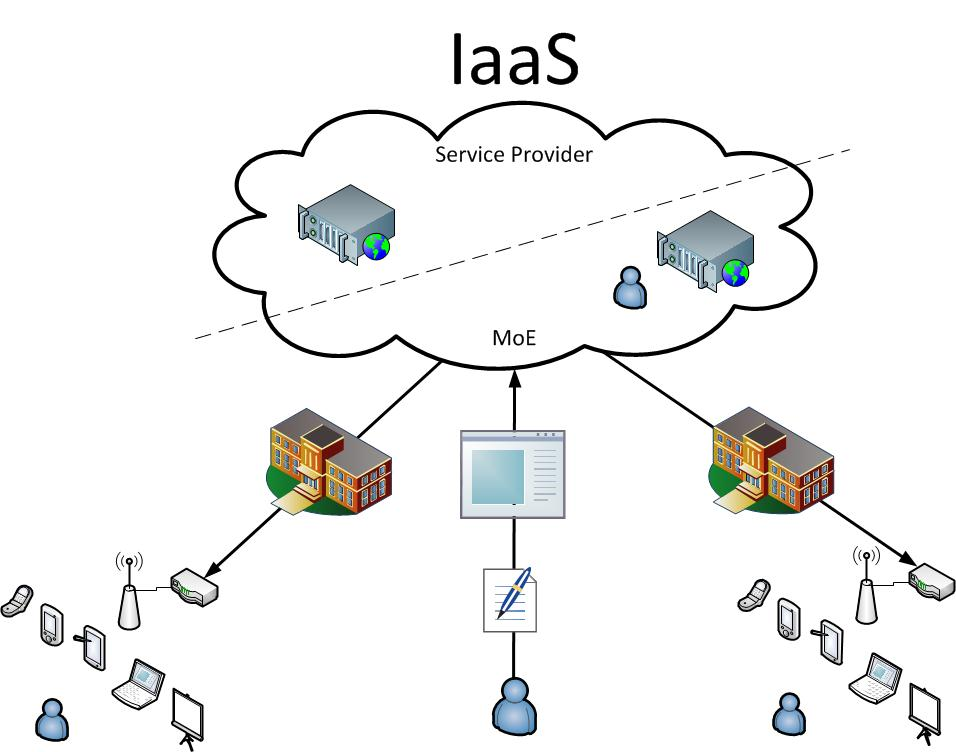
\includegraphics[width=0.7\textwidth]{IaaS.jpg}
	    \caption{ Υπηρεσίες IaaS cloud computing.}
	    \label{fig:iaas}
	\end{figure}
		
		\subsubsection{PaaS}
	
		Η πλατφόρμα σαν υπηρεσία παρέχει στους πελάτες του υπολογιστικού νέφους όλους τους πόρους και τα εργαλεία που απαιτούνται για να έχουν την δυνατότητα να αναπτύξουν, να διαχειριστούν και να τρέξουν εφαρμογές στο διαδίκτυο χωρίς την πολυπλοκότητα και την ανάγκη εγκατάστασης της υποδομής (λογισμικού) που συνήθως συνδέονται με την ανάπτυξη και την έναρξη μιας εφαρμογής. Οι πλατφόρμες σαν υπηρεσίες προσφέρονται σε δύο διαφορετικές μορφές: είτε σαν δημόσιες cloud υπηρεσίες από τον πάροχο, στις οποίες ο χρήστης ελέγχει την ανάπτυξη του λογισμικού και τις ρυθμίσεις διαμόρφωσης, ενώ ο πάροχος εξασφαλίζει το απαραίτητο υπόβαθρο που χρειάζεται η εφαρμογή, είτε σαν λογισμικό, που εγκαθίσταται σε ιδιωτικά κέντρα δεδομένων ή δημόσια υποδομή ως υπηρεσία και διοικείται από εσωτερικά συστήματα πληροφορικής. \cite{Peng2009}
		
		Στο μοντέλο PaaS ο χρήστης δεν ελέγχει την υποκείμενη cloud υποδομή, η οποία συμπεριλαμβάνει το δίκτυο, τους servers, το λειτουργικό σύστημα και τους αποθηκευτικούς χώρους αλλά έχει τον πλήρη έλεγχο στις εγκατεστημένες ή αναπτυγμένες εφαρμογές καθώς και στις ρυθμίσεις των παραμέτρων που γίνονται στο περιβάλλον. Το μοντέλο PaaS βασίζεται σε χρήση της HTML ή Javascript. Υπάρχουν διάφοροι τύποι του μοντέλου PaaS, δημόσιοι, ιδιωτικοί και υβριδικοί. Σε αυτού του τύπου το μοντέλο παροχής υπηρεσιών cloud απαιτούνται δύο επίπεδα προστασίας για τη διασφάλιση της ασφάλειας της ιδιωτικής ζωής. Στο χαμηλότερο επίπεδο του συστήματος, ο πάροχος cloud μπορεί να παρέχει βασικούς μηχανισμούς ασφαλείας, όπως end-to-end κρυπτογράφηση, έλεγχο ταυτότητας και εξουσιοδότηση. Στο υψηλότερο επίπεδο, ο  χρήστης των υπηρεσιών cloud χρειάζεται να καθορίσει τις πολιτικές ελέγχου της πρόσβασης στην εφαρμογή.\cite{Kanagaraj2011}
		
		Στα κύρια πλεονεκτήματα του μοντέλου PaaS συγκαταλέγεται αρχικά το γεγονός ότι επιτρέπει τον προγραμματισμό υψηλού επιπέδου. Επιπροσθέτως, καθιστά την ολική ανάπτυξη μίας εφαρμογής πιο αποτελεσματική, εφόσον έχει ενσωματωμένη δομή, και τη συντήρηση-βελτίωση της πιο εύκολη. Ένα άλλο σημαντικό πλεονέκτημα αποτελεί η υψηλή διαθεσιμότητα, η ελαστικότητα και η ευελιξία που προσφέρει σε συνδυασμό με τις ικανότητες πλήρους αυτοδιαχείρισης και αυτό-κλιμάκωσης της υποδομής και της πλατφόρμας εφαρμογών. Βασικό μειονέκτημα αποτελεί η έλλειψη δια-λειτουργικότητας και η ανικανότητα μεταφοράς της εφαρμογής από έναν πάροχο σε κάποιον άλλον. 

	\begin{figure}[h]
	    \centering
	    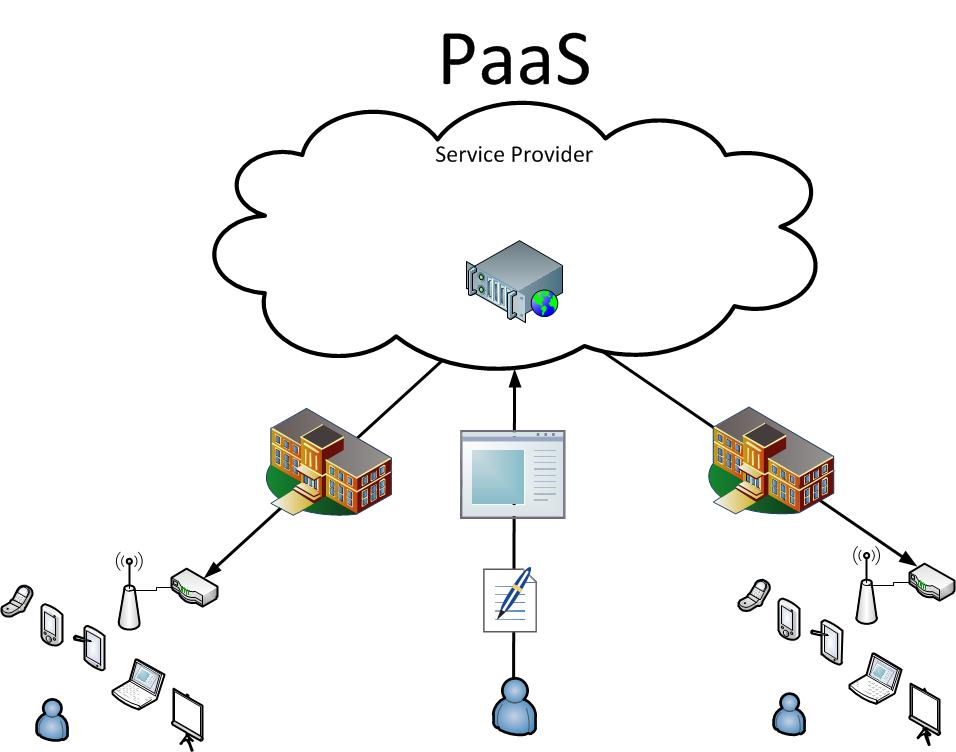
\includegraphics[width=0.7\textwidth]{PaaS.jpg}
	    \caption{Υπηρεσίες PaaS cloud computing.}
	    \label{fig:paas}
	\end{figure}

		\subsubsection{SaaS}
	 
	Το λογισμικό σαν υπηρεσία είναι ένα μοντέλο ανάπτυξης λογισμικού σύμφωνα με το οποίο παρέχονται κατόπιν ζήτησης στον χρήστη εφαρμογές και υπολογιστικοί πόροι. Ουσιαστικά, είναι όλες οι υπηρεσίες του cloud, μέσω των οποίων, οι χρήστες είναι σε θέση να αποκτήσουν πρόσβαση σε εφαρμογές μέσω σύνδεσης στο Internet. Οι εφαρμογές αυτές βρίσκονται στο cloud και μπορούν να χρησιμοποιηθούν για ένα ευρύ φάσμα δραστηριοτήτων, τόσο από εταιρείες όσο και από άτομα. Η χρήση των εφαρμογών αυτών αποτελεί περισσότερο ενοικίαση λογισμικού παρά αγορά του. Με την παραδοσιακές διαδικασία για τις εφαρμογές λογισμικού αρχικά αγοράζεται το λογισμικό ως πακέτο και εγκαθίσταται σε έναν υπολογιστή, ενώ συνήθως οι σχετικές άδειες περιορίζουν τον αριθμό των χρηστών και των συσκευών όπου μπορεί να αναπτυχθεί το λογισμικό. Εν αντιθέσει, οι χρήστες των υπηρεσιών SaaS εγγράφονται στο λογισμικό, χωρίς να το αγοράσουν και επομένως γλιτώνοντας όλη αυτήν τη διαδικασία, και ανανεώνουν τη συνδρομή τους συνήθως σε μηνιαία βάση. 
	
	Οι περισσότεροι χρήστες χρησιμοποιούν έναν λεπτό πελάτη (thin client) για να αποκτήσουν πρόσβαση στις υπηρεσίες SaaS. Οι εταιρικοί χρήστες χρησιμοποιούν τις εφαρμογές που παρέχει ο πάροχος cloud για ανάγκες όπως λογισμικό γραφείου, λογισμικό ανταλλαγής μηνυμάτων,  λογισμικό λογιστικής και τιμολόγησης, λογισμικό παρακολούθησης επιδόσεων, λογισμικό διαχείρισης επιχειρησιακών σχέσεων και άλλα. 
	
	Βασικά πλεονεκτήματα των υπηρεσιών SaaS είναι η ευελιξία και η επεκτασιμότητα που προσφέρουν, καθώς οι χρήστες δεν χρειάζεται να αγοράσουν άλλο λογισμικό ή άλλον server, απλά ενεργοποιούν νέες προσφορές του μοντέλου SaaS. Πολύ σημαντικό είναι επίσης, η υψηλή ποιότητα των υπηρεσιών η υψηλή σταθερότητα και το γεγονός ότι απαιτείται ελάχιστη συντήρηση. Υπάρχει μεγάλο χρονικό κέρδος, καθώς στις υπηρεσίες SaaS το λογισμικό είναι ήδη εγκατεστημένο και ρυθμισμένο και η εφαρμογή μπορεί να διατεθεί στον χρήστη έτοιμη για χρήση. Η πολιτική κοστολόγησης της χρήσης των υπηρεσιών είναι ιδιαίτερα συμφέρουσα συγκριτικά με την αγορά του και πολλές φορές επιτρέπει την χρήση εφαρμογών που σε άλλη περίπτωση θα ήταν απαγορευμένες, λόγω ιδιαίτερα υψηλού κόστους. Θεωρείται αξιόπιστη λύση ασφαλείας, καθώς υιοθετεί SSL (Secure Socket Layer) στις υπηρεσίες του με αποτέλεσμα τα δεδομένα να μεταδίδονται από και προς τον χρήστη με ασφάλεια. Βασικό μειονέκτημα αποτελεί το γεγονός ότι παρέχει πρόσβαση βασισμένη σε ένα δίκτυο που αποτελείται από τις περισσότερο εμπορικές εφαρμογές με αποτέλεσμα να μην μπορεί πάντα κάποιος να βρει το λογισμικό που ψάχνει διαθέσιμο στο SaaS. 
	
		\begin{figure}[h]
	    \centering
	    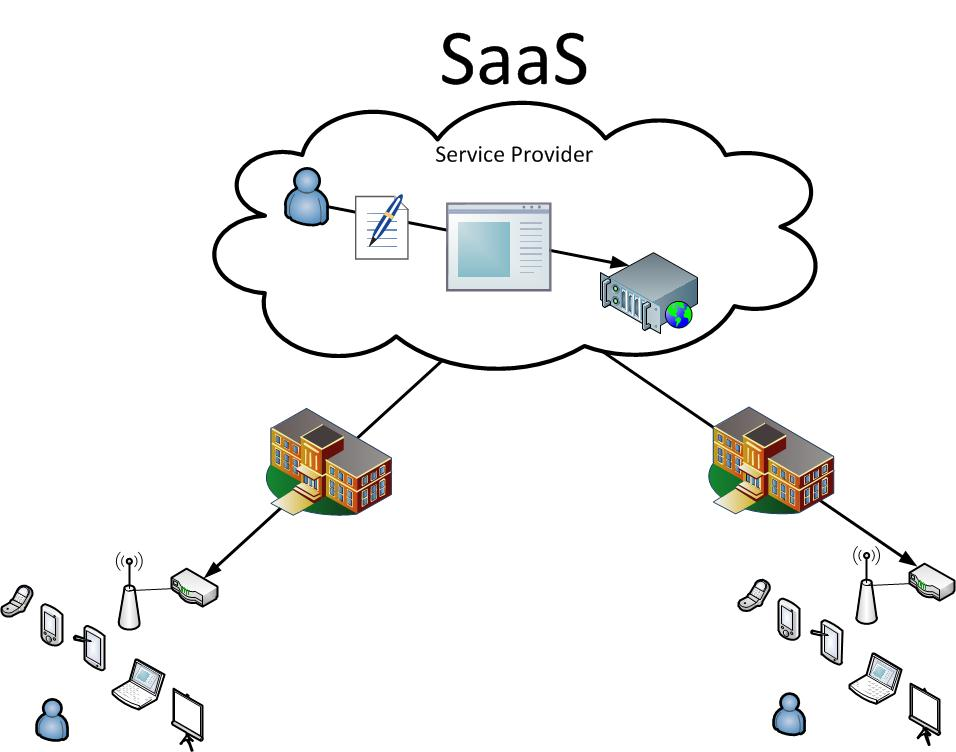
\includegraphics[width=0.7\textwidth]{SaaS.jpg}
	    \caption{Υπηρεσίες SaaS cloud computing.}
	    \label{fig:saas}
	\end{figure}
	
		\subsubsection{BaaS}
 
	
	Η υπηρεσία BaaS είναι ένα μοντέλο που παρέχει στους προγραμματιστές διαδικτυακών εφαρμογών και εφαρμογών για κινητά τηλέφωνα έναν τρόπο εύκολης και γρήγορης διασύνδεσης των εφαρμογών, μέσω παρεχόμενων APIs. Παρέχει υπηρεσίες όπως διαχείριση χρηστών, ειδοποιήσεις (push notifications), κώδικα για server και σύνδεση με υπηρεσίες κοινωνικών δικτύων.  Όλες αυτές οι υπηρεσίες αξιοποιούνται μέσω χρήσης εργαλείων ανάπτυξης λογισμικού (SDKs) και έχουν την δική τους διεπαφή προγραμματισμού εφαρμογών (APIs), που τους επιτρέπει να ενσωματωθούν στις εφαρμογές χωρίς ιδιαίτερο κόπο. Η παροχή ενός σταθερού τρόπου για την διαχείριση των backend δεδομένων συνεπάγεται το γεγονός ότι οι προγραμματιστές δεν χρειάζεται να αναπτύξουν κώδικα backend για κάθε υπηρεσία που χρησιμοποιεί ή έχει πρόσβαση η εφαρμογή τους.

	Ένα από τα κύρια πλεονεκτήματα της χρήσης υπηρεσιών BaaS είναι η τεράστια μείωση του χρόνου ολοκλήρωσης και συντήρησής της εφαρμογής , σε ποσοστό μέχρι και 60\%. Επιπλέον ευνοείται η κλιμάκωση, καθώς το BaaS παρέχει ένα συγκεκριμένο backend το οποίο διαμορφώνει κάποιος εύκολα με βάση τις ανάγκες της εφαρμογής. Η ανάλυση της εφαρμογής γίνεται πιο αποδοτική, καθώς το BaaS διαχειρίζεται όλη τη "κίνηση" που γίνεται μέσα στην εφαρμογή και αναλύει τι συμβαίνει σε αυτήν (ποιοι χρήστες είναι πιο ενεργοί, ποιοι είναι πιο εμπλεκόμενοι κ.λ.π. ). Παρά τα πολλά οφέλη του BaaS, είναι επίσης σημαντικό να ληφθεί υπόψιν η κατασκευή του user-interface (UI), διότι αυτό βρίσκεται σε άμεση επικοινωνία με τους τελικούς χρήστες. Ο ρόλος του UI είναι να συνδέεται η εφαρμογή με άλλα ανεξάρτητα κομμάτια ή με αποκλειστικά APIs που συνδέονται στο backend, κάτι το οποίο με χρήση των υπηρεσιών BaaS δεν είναι δυνατό πολλές φορές καθώς μια εφαρμογή "κλειδώνεται" στον πάροχο.
	
		\begin{figure}[h]
	    \centering
	    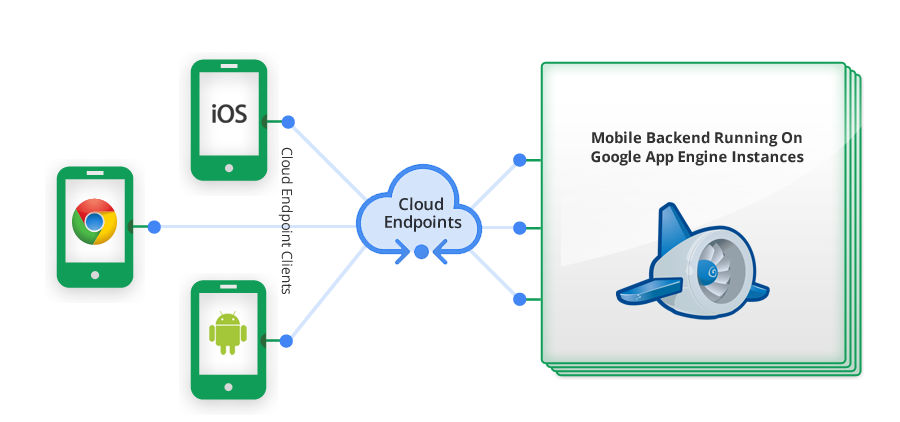
\includegraphics[width=0.7\textwidth]{BaaS.png}
	    \caption{Υπηρεσίες BaaS cloud computing. }
	    \label{fig:baas}
	\end{figure}

	Στην συνέχεια θα αναπτυχθούν τα μοντέλα ανάπτυξης του cloud computing.
	\subsubsection{Public cloud}
	
 
		Το δημόσιο cloud computing είναι ένα μοντέλο μέσω του οποίου οι χρήστες έχουν πρόσβαση στο cloud μέσω διεπαφών που χρησιμοποιούν τα προγράμματα περιήγησης. Ένα cloud καλείται δημόσιο, όταν οι υπηρεσίες του παρέχονται μέσω ενός δημόσιου δικτύου, όπως το Internet και είναι ανοιχτές για δημόσια χρήση. Τα δημόσια cloud παρέχουν υπηρεσίες σε πολλούς πελάτες χρησιμοποιώντας την ίδια διαμοιραζόμενη υποδομή.Πολλά δημόσια cloud δεν χρεώνουν τον χρήστη.
		
		 Οι υπηρεσίες SaaS όπως η αποθήκευση στο cloud και οι online εφαρμογές γραφείου είναι οι υπηρεσίες που βρίσκονται κατά κόρον σε δημόσια cloud. Οι υπηρεσίες υποδομής (IaaS) καθώς και οι πλατφόρμες σαν υπηρεσία (PaaS), κυρίως οι περιπτώσεις του cloud web hosting και των περιβαλλόντων ανάπτυξης, αναπτύσσονται εξίσου συχνά και σε δημόσια και σε ιδιωτικά cloud. Τα δημόσια cloud χρησιμοποιούνται ευρέως σε προσφορές για ιδιώτες οι οποίοι είναι λιγότερο πιθανόν να χρειαστούν το επίπεδο των υποδομών και την ασφάλεια που προσφέρουν τα ιδιωτικά cloud. Ωστόσο, σε πολλές περιπτώσεις οι επιχειρήσεις μπορούν να χρησιμοποιούν δημόσια cloud σε περιπτώσεις που δεν τίθεται θέμα ευαίσθητων δεδομένων (π.χ. webmai, online συνεργασία) για να κάνουν τις λειτουργίες τους πιο αποτελεσματικά \cite{characteristics}.

			Τα βασικά πλεονεκτήματα του δημόσιου cloud είναι:
			\begin{itemize}

			\item Απόλυτη επεκτασιμότητα. Το γεγονός ότι οι υπολογιστικοί πόροι στο cloud είναι "ανεξάντλητοι" και γίνονται διαθέσιμοι ανάλογα με τη ζήτηση έχει ως αποτέλεσμα οι εφαρμογές που τρέχουν σε αυτούς να μπορούν να ανταποκριθούν στις διακυμάνσεις της δραστηριότητας.
			
			\item Υψηλή απόδοση. Τα δημόσια cloud συνεπάγονται υψηλότερα επίπεδα υπολογιστικών πόρων με ταυτόχρονα λιγότερο κόστος. Μερικές προτάσεις μαζικής αγοράς μπορούν ακόμη και να είναι δωρεάν για τον πελάτη και να στηρίζονται στις διαφημίσεις για τα έσοδα τους (Google).
			
			\item Το μοντέλο πληρωμής ανάλογα με τη χρήση. Ο χρήστης είναι σε θέση να αποκτήσει πρόσβαση στους πόρους που χρειάζεται, όποτε θέλει και να πληρώσει μόνο για αυτούς που χρησιμοποιεί αποφεύγοντας τους περιττούς πόρους.

			\item 	Ευελιξία. Υπάρχει ένας τεράστιος αριθμός των IaaS, PaaS και SaaS υπηρεσιών που διατίθενται στην αγορά, οι οποίες ακολουθούν το μοντέλο του δημόσιου cloud και τις οποίες ο χρήστης μπορεί να προσεγγίσει από οποιαδήποτε συσκευή με χρήση Internet. Οι υπηρεσίες αυτές μπορούν να εκπληρώσουν τις περισσότερες υπολογιστικές απαιτήσεις και μπορούν να χρησιμοποιηθούν εξίσου αποτελεσματικά  από ιδιώτες και επιχειρήσεις. 
			
			\item Ανεξαρτησία της τοποθεσίας. Η διαθεσιμότητα των υπηρεσιών του δημόσιου cloud μέσω του Internet, εξασφαλίζει ότι οι υπηρεσίες είναι διαθέσιμες όπου και αν βρίσκεται ο χρήστης. Αυτό το γεγονός πολλές φορές είναι ιδιαίτερα χρήσιμο όπως για παράδειγμα σε περιπτώσεις εταιριών, όπου δίνεται η δυνατότητα για απομακρυσμένη πρόσβαση σε υποδομές πληροφορικής (σε περίπτωση έκτακτης ανάγκης, κ.λ.π.).
			
		\end{itemize}
			
			
	\subsubsection{Private cloud}

	 
	Το ιδιωτικό cloud, είναι ένα μοντέλο το οποίο λειτουργεί αποκλειστικά για έναν οργανισμό, διευθύνεται είτε από τον ίδιο τον οργανισμό είτε από τρίτους και εγκαθίσταται είτε εσωτερικά είτε εξωτερικά. Περιλαμβάνει ένα ξεχωριστό και ασφαλές περιβάλλον με το οποίο μπορούν να αλληλεπιδράσουν οι χρήστες. Τα ιδιωτικά cloud παρέχουν μεγάλη υπολογιστική ισχύ σαν υπηρεσία χρησιμοποιώντας ένα σύνολο από φυσικούς υπολογιστικούς πόρους, οι οποίοι είναι προσβάσιμοι μόνο από έναν οργανισμό, εξασφαλίζοντας περισσότερο έλεγχο και αυξημένη ασφάλεια. Τα δημόσια cloud περιλαμβάνουν πολλούς πελάτες οι οποίοι έχουν πρόσβαση σε εικονικές υπηρεσίες που αντλούν πόρους από την ίδια ομάδα από servers μέσω δημοσίων δικτύων. Τα ιδιωτικά cloud από την άλλη πλευρά, περιλαμβάνουν την οριοθέτηση ενός cloud για την αποκλειστική χρήση από έναν οργανισμού. Παρόλο που χρησιμοποιούνται ξεχωριστοί πόροι, μπορούν να γίνουν προσβάσιμοι μέσω ιδιωτικών γραμμών ή ασφαλών κρυπτογραφημένων συνδέσεων δημόσιου δικτύου \cite{Doelitzscher2011} \cite{Missbach}.
	
	Τα ιδιωτικά cloud είναι κατάλληλα για περιπτώσεις στις οποίες υπάρχει η ανάγκη αποθήκευσης και επεξεργασίας ιδιωτικών ή ευαίσθητων δεδομένων ή η ανάγκη διεξαγωγής ευαίσθητων εργασιών. Για παράδειγμα, μία ιδιωτική cloud υπηρεσία μπορεί να χρησιμοποιηθεί από ένα πληροφοριακό σύστημα που διαχειρίζεται και αποθηκεύει ευαίσθητα ιατρικά δεδομένα και θέλει να επωφεληθεί από τα πλεονεκτήματα του cloud computing στην επιχειρησιακή υποδομή του. 	Υιοθετεί τις βασικές αρχές ασφαλείας, νομοθεσίας και κανονιστικών απαιτήσεων αφού προσφέρει μεγάλο έλεγχο εγκατάστασης και χρήσης στην επιχείρηση που το χρησιμοποιεί. Το ιδιωτικό μοντέλο cloud μοιάζει αρκετά με το μοντέλο των δικτύων τοπικής πρόσβασης (LAN) που χρησιμοποιούταν στο παρελθόν αλλά παρέχει τα επιπλέον πλεονεκτήματα του cloud. Κάποια από τα πλεονεκτήματα του ιδιωτικού cloud είναι:
	
	\begin{itemize}
	
	\item Μεγαλύτερη προστασία και ασφάλεια. Τα δημόσια cloud εφαρμόζουν μηχανισμούς παροχής ασφάλειας, αλλά τα ιδιωτικά cloud με τους αποκλειστικούς φυσικούς πόρους, οι οποίοι επιτρέπουν πρόσβαση μόνο σε συνδέσεις που γίνονται μέσω συγκεκριμένου οργανισμού και προσωπικές ασφαλείς γραμμές εξασφαλίζουν ότι υπάρχει πλήρης ασφάλεια και αξιοπιστία.
	
	\item Περισσότερο έλεγχο με αποτέλεσμα περισσότερη ευελιξία. Εφόσον η πρόσβαση στους πόρους γίνεται μόνο από έναν οργανισμό, αυτός ο οργανισμός έχει την ικανότητα να ρυθμίσει και να διαχειριστεί το cloud όπως επιθυμεί, ώστε να επιτευχθεί το κατάλληλο δίκτυο. 
	
	\item Βελτίωση  της σχέσης κόστους και ενεργειακής απόδοσης. Η εφαρμογή ενός ιδιωτικού μοντέλου cloud μπορεί να συντελέσει στην καλύτερη κατανομή των πόρων σε έναν οργανισμό, εξασφαλίζοντας ότι η διαθεσιμότητα των πόρων ανταποκρίνεται άμεσα και ευέλικτα ανάλογα με τη ζήτηση τους. Παρόλο που είναι πιο ακριβά σε σχέση με τα δημόσια cloud, κάνουν πιο αποτελεσματική χρήση των υπολογιστικών πόρων σε σχέση με τα παραδοσιακά τοπικά δίκτυα (LANs), καθώς ελαχιστοποιείται η επένδυση σε αχρησιμοποίητη παραγωγική ικανότητα. 
	
	\item Βελτιωμένη αξιοπιστία. Ακόμα και αν οι πόροι (servers, δίκτυα, κ.λ.π.) φιλοξενούνται εσωτερικά στον πελάτη, η δημιουργία εικονικών περιβάλλοντων λειτουργικού συνεπάγεται ότι το δίκτυο είναι πιο ανθεκτικό σε επιμέρους αστοχίες από ότι η φυσική υποδομή. 

	\end{itemize}
	
		
		\subsubsection{Community cloud}
		
		Το κοινοτικό cloud είναι ένα μοντέλο νέφους το οποίο μοιράζεται σε διάφορους οργανισμούς και υποστηρίζει μια συγκεκριμένη κοινότητα που έχει κοινά ενδιαφέροντα (ασφάλειας,  συμμόρφωσης, της διεθνούς δικαιοδοσίας, κλπ). Η διαχείριση του νέφους μπορεί να γίνει είτε εσωτερικά  από τον ίδιο τον οργανισμό είτε από τρίτους και υλοποιείται είτε εντός είτε εκτός του οργανισμού. Οι δαπάνες κατανέμονται σε λιγότερους χρήστες από ότι σε ένα δημόσιο cloud (περισσότερους βέβαια από ότι σε ένα ιδιωτικό cloud), και έτσι πραγματοποιούνται μόνο μερικές από τις δυνατότητες εξοικονόμησης κόστους του cloud computing \cite{Briscoe2009} \cite{condori}.
	
	Το κοινοτικό cloud φιλοδοξεί να συνδυάσει την υπολογιστική παροχή των πόρων που διανέμονται από το δίκτυο, τον κατανεμημένο έλεγχο από τα ψηφιακά οικοσυστήματα και τη βιωσιμότητας της "πράσινης" πληροφορικής, με τις περιπτώσεις χρήσης του cloud computing, κάνοντας μεγαλύτερη χρήση των πλεονεκτημάτων της αυτοδιαχείρισης του υπολογιστικού συστήματος. Τα πλεονεκτήματα του κοινοτικού cloud περιλαμβάνουν:
	\begin{itemize}
	
	\item Χαμηλότερο κόστος. Το κόστος της δημιουργίας ενός κοινοτικού cloud έναντι των ιδιωτικών cloud μπορεί να είναι χαμηλότερο λόγω της κατανομή των κοστών σε όλους τους συμμετέχοντες.

	\item Ανάθεση της διαχείρισης σε έναν πάροχο cloud. Το πλεονέκτημα έγκειται στο γεγονός ότι ο πάροχος θα είναι ένας αμερόληπτος τρίτος που δεσμεύεται από σύμβαση και δεν έχει καμία προτίμηση σε κάποιον από τους πελάτες που εμπλέκονται.
	
	\end{itemize}

Βασικό μειονέκτημα αποτελεί το γεγονός ότι το κόστος είναι πολύ υψηλότερο από ότι στα δημόσια cloud \cite{cloudOverview}.

		
		
		
		\subsubsection{Hybrid cloud}
		
		Τα υβριδικά cloud είναι μία ολοκληρωμένη υπηρεσία που αποτελείται από δύο ή περισσότερα cloud (ιδιωτικά, δημόσια ή κοινοτικά) τα οποία παραμένουν ξεχωριστές οντότητες αλλά συνδέονται μεταξύ τους, προσφέροντας τα πλεονεκτήματα των πολλαπλών μοντέλων ανάπτυξης. Μια υπηρεσία υβριδικού cloud ξεπερνά τα όρια του παρόχου σε σχέση με τις άλλες υπηρεσίες cloud,  με αποτέλεσμα να μην μπορεί να κατηγοριοποιηθεί απλά σε μία κατηγορία ιδιωτικών, δημόσιων ή κοινοτικών υπηρεσιών cloud. Με τα υβριδικά cloud μπορεί να επεκταθεί η ικανότητα ή η χωρητικότητα μιας υπηρεσίας μέσω της ένταξης ή της προσαρμογής της με κάποια άλλη υπηρεσία cloud \cite{palwe}.
		
		Η επιλογή υλοποίησης ενός υβριδικού cloud εξαρτάται από έναν αριθμό παραγόντων, όπως οι απαιτήσεις ασφάλειας των δεδομένων και των λειτουργιών πάνω σε αυτά, το επίπεδο ελέγχου που απαιτείται, καθώς και τις εφαρμογές που χρησιμοποιεί ο χρήστης. Όλες οι υπηρεσίες του cloud computing προσφέρουν βελτίωση της αποτελεσματικότητας, αλλά οι υπηρεσίες των δημόσιων cloud υπερτερούν σε σχέση με αυτές των ιδιωτικών λόγω χαμηλότερου κόστους και καλύτερης κλιμάκωσης. Ως εκ τούτου, ένας οργανισμός μπορεί να μεγιστοποιήσει την αποτελεσματικότητα του χρησιμοποιώντας υπηρεσίες από δημόσια cloud για όλες τις μη-ευαίσθητες λειτουργίες, στηριζόμενος σε χρήση ιδιωτικού cloud μόνο όταν κρίνεται τελείως απαραίτητο, και διασφαλίζοντας ότι όλες οι πλατφόρμες συνεργάζονται άψογα μεταξύ τους \cite{Zhou2013}.
		
		Το εξειδικευμένο μοντέλο του υβριδικού cloud, το οποίο είναι χτισμένο πάνω σε ετερογενές hardware, ονομάζεται "Cross-platform Hybrid Cloud". Συνήθως χρησιμοποιούνται διαφορετικές αρχιτεκτονικές επεξεργαστών, για παράδειγμα, x86-64 και ARM. Οι χρήστες μπορούν να αναπτύξουν εφαρμογές με πλήρη διαφάνεια, χωρίς να γνωρίζουν την πολυμορφία του υλικού του cloud. Αυτό το είδος cloud έχει προκύπτει από την αύξηση των βασισμένων σε ARM system-on-chip αρχιτεκτονικών για servers.
		
		Ένα ειδικά διαμορφωμένο υβριδικό cloud, προσφέρει τα εξής πλεονεκτήματα:
		
		\begin{itemize}

		\item Επεκτασιμότητα. Ενώ τα ιδιωτικά cloud προσφέρουν δυνατότητα κλιμάκωσης η οποία εξαρτάται από τις ρυθμίσεις τους (όπως το αν φιλοξενούνται εσωτερικά ή εξωτερικά), οι υπηρεσίες των δημοσίων cloud computing προσφέρουν πολύ αυξημένες δυνατότητες επεκτασιμότητας, διότι οι πόροι τους προέρχονται από μεγαλύτερες υποδομές. Υλοποιώντας τις μη-ευαίσθητες λειτουργίες σε δημόσιο cloud μπορεί ένας οργανισμός να επωφεληθεί από την επεκτασιμότητα του δημόσιου cloud και ταυτόχρονα να μειώσει τις απαιτήσεις στο ιδιωτικό cloud.
		
		\item Εξοικονόμηση κόστους. Τα δημόσια cloud  προσφέρουν με χρήση υπηρεσιών (όπως η κεντρική διαχείριση) μεγαλύτερη αποδοτικότητα κόστους, από τα ιδιωτικά cloud. Ως εκ τούτου, τα υβριδικά σύννεφα επιτρέπουν στους οργανισμούς να έχουν πρόσβαση σε αυτές τις συμφέρουσες υπηρεσίες για όσες από τις λειτουργίες τους είναι εφικτό, διατηρώντας ωστόσο τις ευαίσθητες λειτουργίες ασφαλείς στο ιδιωτικό cloud.

		\item Ασφάλεια. Το ιδιωτικό cloud του μοντέλου υβριδικού cloud παρέχει την απαραίτητη ασφάλεια για τις ευαίσθητες λειτουργίες και επιπλέον σε πολλές περιπτώσεις τηρεί τις προϋποθέσεις για τον χειρισμό και την αποθήκευση δεδομένων.

		\item Ευελιξία. Η διαθεσιμότητα τόσο των ασφαλών πόρων του ιδιωτικού cloud και όσο και των οικονομικότερων των δημοσίων cloud, παρέχει στους οργανισμούς περισσότερες ευκαιρίες για να εξερευνήσουν διαφορετικές επιχειρησιακές κατευθύνσεις.
		\end{itemize} 

		\subsection{NodeJs}
	
		Το Node.js, ή απλούστερα Node, είναι μια πλατφόρμα που μας επιτρέπει να γράψουμε JavaScript στην πλευρά του εξυπηρετητή (server-side JavaScript). Από το 2009, που δημιουργήθηκε, μέχρι σήμερα η πλατφόρμα έχει εξελιχθεί ραγδαία και χρησιμοποιείται σε πολλές μεγάλες εφαρμογές. Αποτελεί αυτήν την στιγμή το δεύτερο σε επισκεψιμότητα πρότζεκτ στο GitHub και έχει παραπάνω από 90000 πακέτα (modules) που έχουν δημοσιευτεί στον διαχειριστή πακέτων του Node (Node Package Manager, NPM). Οι NodeJs εφαρμογές είναι γραμμένες σε JavaScript και μπορούν να εκτελεστούν σε OS X, Microsoft Windows, Linux, FreeBSD, NonStop, IBM AIX, IBM System z και IBM i. Το πρότζεκτ του Node φιλοξενείται και υποστηρίζεται από το Node.js Foundation, ένα συλλογικό έργο του Linux Foundation \cite{Tilkov2010}.

		Το Node είναι μια οδηγούμενη από γεγονότα (event-driven) πλατφόρμα,  στην οποία μια διεργασία σε αντίθεση με τα περισσότερα σύγχρονα περιβάλλοντα ανάπτυξης εφαρμογών  δεν στηρίζεται στην πολυνηματικότητα αλλά χρησιμοποιεί λειτουργίες εισόδου/εξόδου χωρίς αναμονή (non blocking I/O), ή ισοδύναμα χρησιμοποιεί ασύγχρονη Ε/Ε (asynchronous I/O) . Αυτό έχει ως σκοπό να αυξήσει την απόδοση και τη δυνατότητα κλιμάκωσης (scalability) των διαδικτυακών εφαρμογών πραγματικού χρόνου. Το Node χρησιμοποιεί την V8, μια εικονική μηχανή που αναπτύχθηκε από τη Google για τον Google Chrome και τρέχει κώδικα JavaScript. Η V8 δίνει στο Node μεγάλη αύξηση στην απόδοση, καθώς κάνει απευθείας μεταγλώττιση σε γλώσσα μηχανής αντί να εκτελεί bytecode ή να χρησιμοποιεί διερμηνευτή (interpreter).

	Το Node επιτρέπει τη δημιουργία web servers και εργαλείων δικτύωσης με χρήση της γλώσσας JavaScript και μια συλλογή από πακέτα (modules), τα οποία χειρίζονται διάφορες λειτουργίες του πυρήνα \cite{node}. Τα πακέτα αυτά χειρίζονται το σύστημα αρχείων Ε/Ε, το σύστημα δικτύωσης (HTTP, TCP, UDP, DNS, ή TLS / SSL), τα δυαδικά δεδομένα (buffers)] και άλλες βασικές λειτουργίες. Τα πακέτα του NodeJs χρησιμοποιούν ένα API το οποίο έχει σχεδιαστεί για να μειώσει την πολυπλοκότητα της ανάπτυξης εφαρμογών για διακομιστή.

	Χρησιμοποιείται κυρίως για την κατασκευή προγραμμάτων δικτύου, όπως διακομιστές δικτύου (web servers), γεγονός που το καθιστά παρόμοιο με την PHP και την Python. Η μεγαλύτερη διαφορά μεταξύ PHP και Node είναι ότι η PHP είναι μια γλώσσα με αναμονή, όπου η εκτέλεση των εντολών προχωρά μόνο όταν έχουν ολοκληρωθεί οι προηγούμενες, ενώ στο Node  οι εντολές εκτελούνται παράλληλα και χρησιμοποιούνται  κλήσεις με επιστροφή (callbacks) για να σηματοδοτηθεί η ολοκλήρωση. Το Node υλοποιεί οδηγούμενο από γεγονότα προγραμματισμό για διαδικτυακές εφαρμογές σε JavaScript. Οι προγραμματιστές μπορούν να δημιουργήσουν εξαιρετικά επεκτάσιμους servers χωρίς τη χρήση νημάτων, χρησιμοποιώντας ένα απλοποιημένο οδηγούμενο από γεγονότα μοντέλο προγραμματισμού που χρησιμοποιεί κλήσεις επιστροφή για να σηματοδοτήσει την ολοκλήρωση ενός στόχου\cite{surenda}.

\subsubsection{Javascript}

		Η JavaScript αναπτύχθηκε αρχικά από τον Brendan Eich του Netscape και ονομαζόταν Μόκα, η οποία αργότερα μετονομάστηκε σε LiveScript, και τελικά σε JavaScript. LiveScript ήταν το επίσημο όνομα για τη γλώσσα, όταν εισήχθη για πρώτη φορά σε beta εκδόσεις του Netscape Navigator 2,0 αλλά μετονομάστηκε σε JavaScript σε μια κοινή ανακοίνωση με την Sun Microsystems όταν προοριζόταν να αναπτυχθεί στη νέα έκδοση του Netscape Navigator 2.0B3.

		H JavaScript, επίσης γνωστή ως ECMAScript, είναι μία πρότυπη αντικειμενοστραφής scripting γλώσσα η οποία είναι δυναμική και έχει πρώτης τάξεως λειτουργίες. Η JavaScript είναι μια εφαρμογή του προτύπου γλώσσας ECMAScript και χρησιμοποιείται κυρίως με τη μορφή client-side, όπου υλοποιείται ως μέρος ενός web browser, ώστε να παρέχεται ενισχυμένη διεπαφή χρηστών και δυναμικές ιστοσελίδες. Αυτό επιτρέπει την πρόσβαση μέσω προγραμματισμού στα υπολογιστικά αντικείμενα μέσα σε ένα περιβάλλον υποδοχής. Η JavaScript χρησιμοποιεί σύνταξη επηρεασμένη από αυτή της C. Πολλά ονόματα και συμβάσεις ονοματολογίας έχουν αντιγραφεί από τη Java, αλλά οι δύο γλώσσες είναι διαφορετικές και έχουν πολύ διαφορετική σημασιολογία. Οι βασικές αρχές σχεδιασμού στο πλαίσιο της JavaScript, λαμβάνονται από Self και Scheme γλώσσες προγραμματισμού. Είναι μια γλώσσα συγγραφής σεναρίων (scripting language) για την προσθήκη διαδραστικότητας (interactivity) σε ιστοσελίδες. 
	
		Με την JavaScript μπορούμε να φτιάξουμε σενάρια που να εκτελούν αυτόματες εργασίες, για παράδειγμα όταν μια σελίδα του Web ανοίγει ή κλείνει. Επίσης μπορούμε να χρησιμοποιήσουμε την Javascript για να εκτελέσει ενέργειες που να ανταποκρίνονται σε ένα συγκεκριμένο γεγονός. Για παράδειγμα, όταν ο χρήστης επιλέγει ένα κουμπί, έναν σύνδεσμο ή όταν επιλέγει να εστιάσει από ένα στοιχείο μιας φόρμας σε ένα άλλο στοιχείο της, εκτελείται κώδικας Javascript. 

		Κάθε φυλλομετρητής υλοποιεί τον δικό του διερμηνευτή για την JavaScript (συνήθως καλείται μηχανή JavaScript), ο οποίος μάλιστα είναι και καθοριστικής σημασίας για την απόδοση του φυλλομετρητή όσον αφορά στη συμβατότητα, σταθερότητα, ταχύτητα και ασφάλεια. Συνήθως ο κώδικας JavaScript διερμηνεύεται, δε μεταγλωττίζεται. Εντούτοις για να βελτιωθεί η απόδοση, υπάρχουν φυλλομετρητές που ακολουθούν μεθόδους just-in-time μεταγλώττισης, όπως ο Google Chrome με μια καινοτόμο μηχανή JavaScript, την V8.
		
		Η σύνταξη JavaScript είναι κοινή μεταξύ των διάφορων φυλλομετρητών, παρόλο που υπάρχουν διαφορές στην ονοματολογία των βασικών μεθόδων. Η σύνταξη θυμίζει php, με τη διαφορά ότι δεν χρησιμοποιείται το χαρακτηριστικό «\$» στα ονόματα των μεταβλητών. Πρόκειται για μια γλώσσα χαλαρών τύπων όπου οι μεταβλητές μπορούν να αλλάξουν τύπο δυναμικά. Αλφαριθμητικά μεταβλητού μεγέθους υποστηρίζονται εγγενώς. Για τη δήλωση μιας μεταβλητής χρησιμοποιείται η λέξη-κλειδί "var" ενώ για τον ορισμό συνάρτησης χρησιμοποιείται η λέξη "function" και δεν απαιτείται να δηλωθεί ο τύπος του αποτελέσματος. Δεν υπάρχουν δείκτες, ενώ υποστηρίζονται τάξεις. 

\subsubsection{Javascript στον Εξυπηρετητή (server-side Javascript)}

 
 Μέχρι πρόσφατα η Javascript χρησιμοποιούνταν μόνο στο front-end των προγραμμάτων περιήγησης και οι προγραμματιστές ήταν υποχρεωμένοι να χρησιμοποιούν άλλες γλώσσες για τον προγραμματισμό στον εξυπηρετητή (server) και στον εξυπηρετούμενο (client). Το γεγονός ότι το Node μας δίνει τη δυνατότητα να χρησιμοποιήσουμε την ίδια γλώσσα και στις δύο άκρες, απλουστεύει σημαντικά την ανάπτυξη των διαδικτυακών εφαρμογών.  Με αυτόν τον τρόπο, το μόνο προαπαιτούμενο για να αναπτύξει κανείς μια διαδικτυακή εφαρμογή είναι η γνώση Javascript. Εκτός από τη μεγάλη διευκόλυνση που προσφέρει, το γεγονός ότι χρησιμοποιούμε Javascript και στις δύο πλευρές συντελεί σημαντικά και στην αύξηση της απόδοσης των διαδικτυακών εφαρμογών. Με χρήση του προγράμματος περιήγησης Google Chrome, η ταχύτητα με την οποία εκτελείται η JavaScript αυξάνεται με τρομερά ταχείς ρυθμούς.

Η JavaScript δεν παρέχει κάποια βιβλιοθήκη για λειτουργίες Ε/Ε με σύγχρονο τρόπο και εξαιτίας αυτού  οι λειτουργίες που παρέχονται στην πλατφόρμα Node είναι χωρίς αναμονή (non blocking). Οι συναρτήσεις στην JavaScript αποτελούν αντικείμενα πρώτης τάξης (first-class functions). Αυτό σημαίνει ότι η γλώσσα υποστηρίζει το πέρασμα μιας συνάρτησης σαν παράμετρο σε μια άλλη συνάρτηση και την επιστροφή μιας συνάρτησης σαν αποτέλεσμα από μια άλλη συνάρτηση. Επιπλέον, η JavaScript παρέχει το μοτίβο κλεισίματος (closure pattern). Με αυτόν τον τρόπο οι συναρτήσεις επιστρεφόμενης κλήσης (callback functions) έχουν την ιδιότητα να κρατάνε στοιχεία και να ξέρουν το περιβάλλον λειτουργίας στο οποίο δηλώθηκαν και τις μεταβλητές που υπήρχαν σε αυτό το περιβάλλον. Το Node στηρίζεται στα παραπάνω δύο χαρακτηριστικά της Javascript.

\subsubsection{Νήματα, μονονηματικό μοντέλο και πολυνηματισμός}

		Οι παραδοσιακές προγραμματιστικές τεχνικές παγώνουν την συνέχεια της εκτέλεσης μιας διεργασίας όταν μεσολαβήσει μια διακοπή ή μια λειτουργία E/E μέχρι αυτή να ολοκληρωθεί. Στις διαδικτυακές εφαρμογές όμως ο χρήστης πρέπει να μπορεί να αλληλεπιδράσει με το σύστημα και να μην αναμένει την ολοκλήρωση της κάθε λειτουργίας Ε/Ε. Μία μέθοδος που δημιουργήθηκε για να αντιμετωπίσει αυτό το πρόβλημα είναι η χρήση νημάτων. Νήμα (thread) είναι ένα είδος ελαφριάς διεργασίας που μπορεί να χρησιμοποιήσει την κεντρική μονάδα επεξεργασίας και μοιράζεται τη μνήμη με κάθε άλλο νήμα μέσα σε μια διεργασία. Όσο ένα νήμα βρίσκεται σε αναμονή ώσπου μια λειτουργία Ε/Ε να ολοκληρωθεί, ένα άλλο νήμα της ίδιας διεργασίας μπορεί να χρησιμοποιήσει την κεντρική μονάδα επεξεργασίας. Μόλις η λειτουργία Ε/Ε ολοκληρωθεί, η εκτέλεση περνάει πάλι στο πρώτο νήμα και το δεύτερο κοιμάται. Η διαδικασία αυτή ονομάζεται πολυνηματισμός.
		
		
	\begin{figure}[h]
	    \centering
	    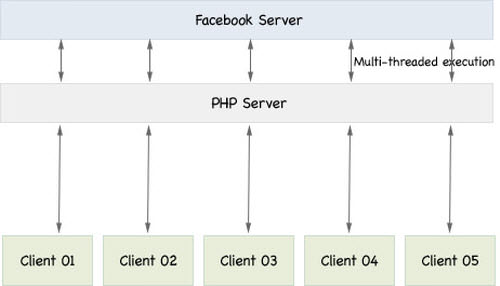
\includegraphics[width=0.7\textwidth]{multi-threaded.jpg}
	    \caption{Πολυνηματικό Μοντέλο.}
	    \label{fig:multi}
	\end{figure}
	
	
	
		 Ο πολυνηματισμός παρόλο που λύνει το πρόβλημα της απόδοσης και των μεγάλων νεκρών διαστημάτων της πρώτης υλοποίησης παρουσιάζει κάποια προβλήματα. Αρχικά απαιτεί πολύ χρόνο εργασίας από τον προγραμματιστή καθώς και τη χρήση εξειδικευμένων λύσεων συγχρονισμού των νημάτων, όπως κλειδώματα (locks) και σημαφόρους (semaphores), με σκοπό να μην πραγματοποιηθεί ταυτόχρονη πρόσβαση δύο νημάτων στο ίδιο σημείο της μνήμης, η οποία θα έχει ως αποτέλεσμα ασυνέπειες  \cite{silberschatz}. Τέτοιου είδους λάθη (bugs) δεν είναι πάντα εύκολο να προβλεφθούν και πολλές φορές συμβαίνουν τυχαία και είναι πολύ δύσκολος ο εντοπισμός τους. Ένα άλλο μειονέκτημα του μοντέλου του πολυνηματισμού είναι ότι το μοντέλο  δεν κλιμακώνει ιδιαίτερα καλά καθώς ο αριθμός των χρηστών αυξάνεται. Η διαχείριση όλων αυτών των νημάτων είναι ένα μεγάλο βάρος για το λειτουργικό σύστημα, τόσο λόγω των απαιτήσεων μνήμης, όσο και λόγω της εναλλαγής περιβάλλοντος λειτουργίας. Η εναλλαγή της ΚΜΕ ανάμεσα στα νήματα απαιτεί την αποθήκευση της κατάστασης του τρέχοντος νήματος και την επαναφορά της κατάστασης του προς εκτέλεσης νήματος. 
		
		 
		 Το Node για να αντιμετωπίσει όλα αυτά τα προβλήματα, υιοθετεί μία διαφορετική προσέγγιση δημιουργώντας μόνο ένα νήμα το οποίο χειρίζεται όλες τις λειτουργίες Ε/Ε. Με αυτόν τον τρόπο επιτυγχάνει υψηλά επίπεδα κλιμάκωσης, που μπορεί να φτάσουν τις ένα εκατομμύριο ταυτόχρονες συνδέσεις. Στο σχήμα \ref{fig:single} φαίνεται ένα παράδειγμα από το μονονηματικό μοντέλο του NodeJs.
		 
			 \begin{figure}[h]
	    \centering
	    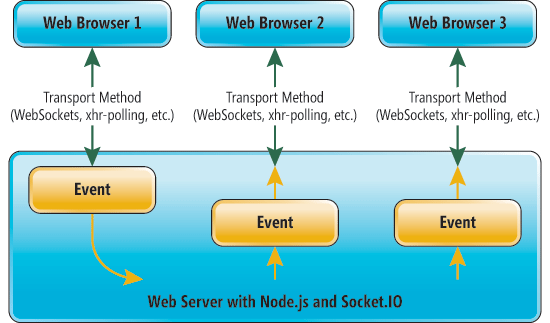
\includegraphics[width=0.7\textwidth]{single.png}
	    \caption{ Το μονονηματικό μοντέλο του NodeJs.}
	    \label{fig:single}
	\end{figure} 

\subsubsection{Event-driven model}		 

		O οδηγούμενος από τα γεγονότα (event-driven) προγραμματισμός είναι ένα προγραμματιστικό μοντέλο όπου η ροή της εκτέλεσης ``οδηγείται'' από γεγονότα. Τα γεγονότα αυτά τα χειρίζονται είτε οι επιστρεφόμενες κλήσεις των γεγονότων είτε οι χειριστές συμβάντος. Μια επιστρεφόμενη κλήση είναι μια συνάρτηση η οποία καλείται όταν συμβαίνει ένα συγκεκριμένο γεγονός. Στα πλαίσια του εξυπηρετητή το γεγονός στο οποίο αναφερόμαστε συνήθως αποτελεί η ολοκλήρωση μιας λειτουργίας Ε/Ε. Για παράδειγμα, σε μια γραφική διεπαφή χρήστη έχουμε ως γεγονότα τα πατήματα πλήκτρων ή επιλογών με το ποντίκι.
		
		Στις περιπτώσεις που οι λειτουργίες Ε/Ε επιστρέφουν μία συνάρτηση και όχι απλά μία τιμή έχουμε το μοντέλο του ασύγχρονου ή οδηγούμενου από γεγονότα προγραμματισμού. Έτσι επιτυγχάνεται η παραλληλοποίηση των Ε/Ε λειτουργιών,ενώ κάθε φορά η συνάρτηση επιστρεφόμενης κλήσης ενημερώνει για την ολοκλήρωση της αντίστοιχης λειτουργίας. Η JavaScript ανήκει σε αυτό το είδος προγραμματισμού. Η JavaScript υποστηρίζει επιπλέον το μοτίβο κλεισίματος (closure pattern) καθώς και το πέρασμα συναρτήσεων σαν παραμέτρους σε άλλη συνάρτηση (first-class functions).
		

		Ο οδηγούμενος από τα γεγονότα προγραμματισμός συνοδεύεται από έναν βρόχο γεγονότων (event loop). Ο βρόχος γεγονότων είναι ένα loop το οποίο σε κάθε επανάληψη ανιχνεύει γεγονότα και ενεργοποιεί τον αντίστοιχο χειριστή συμβάντος. Ουσιαστικά κοιτάει σε κάθε επανάληψη ποια λειτουργία Ε/Ε έχει ολοκληρωθεί και καλεί την αντίστοιχη συνάρτηση επιστρεφόμενης κλήσης. Ο βρόχος γεγονότων υλοποιείται από ένα νήμα μέσα σε μια διεργασία και με βάση όσα αναφέρθηκαν για τα νήματα εύκολα προκύπτει ότι κάθε χρονική στιγμή τρέχει το πολύ ένα νήμα, που στην περιπτωσή μας είναι ένας διαχειριστής γεγονότος, και ότι κάθε διαχειριστής γεγονότος τρέχει μέχρι να ολοκληρωθεί χωρίς διακοπή.
		
		\subsubsection{Ο Διαχειριστής Πακέτων του Node (Node Package Manager ,NPM)}
		

		Ο διαχειριστής πακέτων του Node (Node Package Manager ή NPM) παρέχει την δυνατότητα να κατεβάσουμε, να εγκαταστήσουμε και να τρέξουμε στην εφαρμογή μας πακέτα (modules) τρίτων. H εγκατάσταση του διαχειριστή  πακέτων πραγματοποιείται αυτόματα όταν εγκαθιστούμε την πλατφόρμα του Node. Μετά την εγκατάσταση του Node, έχουμε πρόσβαση σε κάποια ενσωματωμένα πακέτα, τα οποία μας παρέχουν κάποιες διεπαφές εφαρμογών χαμηλού επιπέδου (low-level APIs) ώστε να μπορούμε να υλοποιήσουμε κάποιες βασικές λειτουργίες που χρειάζονται οι εφαρμογές. Αυτά τα πακέτα ονομάζονται ως ο πυρήνας του NodeJs . Στα πλαίσια σύνθετων εφαρμογών είναι σχεδόν απαραίτητο να συμπεριλάβουμε πακέτα τρίτων.


		Το σύνολο όλων των πακέτων που έχουν φτιάξει και δημοσιοποιήσει οι προγραμματιστές διατηρείται σε μία κεντρική αποθήκη από τον διαχειριστή πακέτων του Node. Ο διαχειριστής πακέτων παρέχει ένα εργαλείο γραμμής-εντολών (command-line tool), όπου ο χρήστης μπορεί να εγκαθιστά και να διαχειρίζεται τα πακέτα αυτά. H αναζήτηση τέτοιων πακέτων μπορεί να πραγματοποιηθεί είτε μέσω της γραμμής εντολών είτε μέσω της σελίδας www.npmjs.org. Σε αυτήν την σελίδα παρουσιάζονται και διάφορα στατιστικά στοιχεία, όπως πόσα πακέτα υπάρχουν συνολικά, από ποια πακέτα εξαρτώνται περισσότερο άλλα πακέτα κ.λ.π. \cite{cantelon}		
				
	\subsubsection{Ο Εξυπηρετητής (Server)}
	
		To NodeJs κάνει την δημιουργία διαφόρων τύπων εξυπηρετητών (servers) μια πολύ εύκολη διαδικασία καθώς στο NodeJs ο εξυπηρετητής και η εφαρμογή είναι το ίδιο.

		
	\subsection{Βάση Δεδομένων}
	Στο παρόν κεφάλαιο κάνουμε μια σύντομη αναφορά στα διάφορα συστήματα βάσεων δεδομένων τύπου NoSQL, τα πλεονεκτήματα τους καθώς και τις εφαρμογές για τις οποίες ενδείκνυται η χρήση τους.
	
	Η ιδέα ενός συστήματος βάσης δεδομένων τύπου NoSQL παρουσιάστηκε για πρώτη φορά το 1998 χωρίς να προχωρήσει όμως ιδιαίτερα και επανήλθε πάλι στο προσκήνιο το 2009, όταν και αναπτύχθηκαν αρκετές NoSQL λύσεις \cite{5993686} \cite{Codd:1970:RMD:362384.362685}. Η διαδικασία απόδοσης κάποιου συγκεκριμένου ορισμού για τον όρο NoSQL δεν αποτελεί απλή διαδικασία, δεδομένου ότι δεν αναφέρεται σε ένα συγκεκριμένο σύστημα διαχείρισης βάσεων δεδομένων, αλλά αποτελεί έναν γενικό όρο που περικλείει πολλά συστήματα βάσεων δεδομένων.
	
	Στον τομέα της επιστήμης των υπολογιστών όταν αναφερόμαστε στον όρο NoSQL (Not Only SQL), μιλάμε για ένα ευρύ φάσμα συστημάτων διαχείρισης βάσεων δεδομένων τα οποία παρέχουν ένα μηχανισμό προς αποθήκευση και ανάκτηση δεδομένων διαφορετικό από αυτό του σχεσιακού μοντέλου των κλασσικών RDBMS (Relational database management system)\cite{Cattell:2011:SSN:1978915.1978919}\cite{6106531}. Τα συστήματα NoSQL ξεφεύγουν από την παραδοσιακή χρήση πινάκων για την οργάνωση των δεδομένων και χρησιμοποιούν διαφορετικές δομές οργάνωσης, όπως αυτή του κλειδιού-τιμής. Επιπροσθέτως η επεξεργασίά αυτών των δεδομένων δεν γίνεται με χρήση ερωτημάτων SQL όπως έχουμε συνηθίσει. Λόγω των εγγενών διαφορών μεταξύ των δύο αυτών συστημάτων, κάποιες λειτουργίες είναι ταχύτερες στα συστήματα NoSQL ενώ κάποιες άλλες στα συστήματα σχεσιακών βάσεων δεδομένων.
	
	\begin{figure}[h]
	    \centering
	    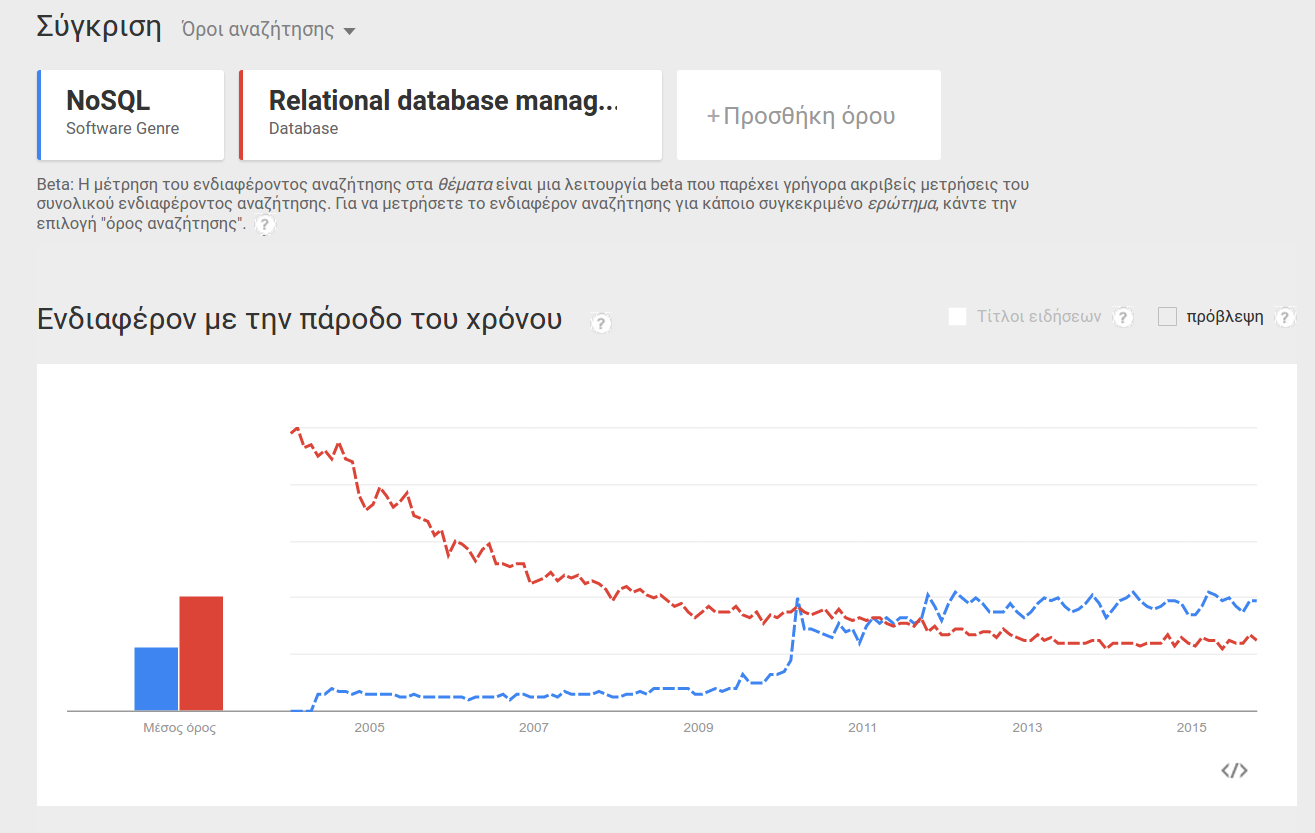
\includegraphics[width=1\textwidth]{nosql_vs_rdbms.png}
	    \caption{Τάση αναζητήσεων Google για NoSQL σε σύγκριση με RDBMS.}
	    \label{fig:NoSQL_vs_rdbms_google}
	\end{figure}
	
	Η χρήση των βάσεων δεδομένων τύπου NoSQL έχει γνωρίσει ραγδαία αύξηση τα τελευταία χρόνια σε εφαρμογές big data καθώς και σε εφαρμογές πραγματικού χρόνου. Αποκαλούνται με τον όρο Not Only SQL για να δοθεί έμφαση στο γεγονός ότι οι δύο τεχνολογίες δεν είναι αμοιβαία αποκλειόμενες. Έχουν τη δυνατότητα να συνυπάρχουν, κρατώντας τα δυνατά σημεία της κάθε μιας, προσφέροντας σε διαφορετικές καταστάσεις διαφορετικές υπηρεσίες. Οι βάσεις δεδομένων τύπου NoSQL χρησιμοποιούνται από εταιρείες κολοσσούς του τεχνολογικού τομέα όπως το Facebook, Amazon, Google, LinkedIn\cite{5993686}. Ο όγκος των δεδομένων που διαχειρίζονται τέτοιες εταιρείες είναι της τάξης πολλών petabyte και επομένως θα ήταν αδύνατη η κλιμάκωσή τους με κάποιο σχεσιακό σύστημα ΒΔ. Κι αυτό γιατί οι σχεσιακές ΒΔ συναντούν περιορισμούς όσον αφορά την αντιμετώπιση προβλημάτων όπως είναι η εξόρυξη δεδομένων, το Web 2.0, το cloud computing, τα μη γραμμικά σε εκτέλεση ερωτήματα κ.τ.λ.
	
	\begin{figure}[h]
	    \centering
	    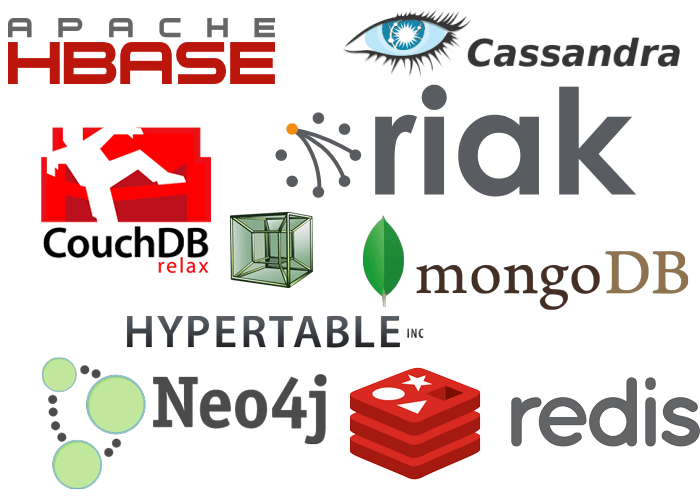
\includegraphics[width=0.7\textwidth]{NoSQL-DBs.png}
	    \caption{Δημοφιλές βάσεις δεδομένων τύπου NoSQL.}
	    \label{fig:NoSQL-DBs}
	\end{figure}
	
	Τα NoSQL συστήματα δεν εμφανίστηκαν για να αντικαταστήσουν τα σχεσιακά, αλλά για να τα συμπληρώσουν. Όπως και σε πολλές άλλες περιπτώσεις έτσι και εδώ, το ζητούμενο είναι να γίνει η επιλογή του κατάλληλου εργαλείου για τη λύση του κάθε προβλήματος. Έτσι στις περισσότερες περιπτώσεις είναι απαραίτητο να γίνει μια εκτίμηση των δυνατοτήτων των διαθέσιμων συστημάτων και στη συνέχεια να υλοποιηθεί ένας συνδυασμός τους ώστε κάθε επιμέρους ανάγκη να καλύπτεται από το σύστημα που της ταιριάζει καλύτερα. Έτσι, όσο τα δεδομένα του διαδικτύου αυξάνονται με εκθετικούς ρυθμούς, τόσο πιο πολλές θα είναι και οι περιπτώσεις όπου θα καθίσταται καλή επιλογή η χρήση τους. Η ανάπτυξη των NoSQL συστημάτων είναι πολύ γρήγορη τα τελευταία χρόνια. Τη στιγμή της συγγραφής της παρούσας διπλωματικής εργασίας, η λίστα με τις NoSQL βάσεις δεδομένων περιλαμβάνει περίπου 225 καταχωρήσεις όταν πριν από τέσσερα χρόνια οι καταχωρήσεις έφταναν τις 35\cite{numberOfNoSQL}.
		
		\subsubsection{Τύποι NoSQL}
		Όπως αναφέραμε και προηγουμένως με τον όρο NoSQL αναφερόμαστε σε ένα ευρύ φάσμα τεχνολογιών. Στην παρούσα ενότητα θα κάνουμε μια σύντομη παρουσίαση των πιο διαδεδομένων τεχνολογιών.
		
		\subsubsection{Key-value Stores (Αποθήκες κλειδιών-τιμών)}
		Το μοντέλο κλειδιού - τιμής είναι το πιο απλό από όλες τις κατηγορίες που εξετάζουμε. Τα δεδομένα αποθηκεύονται σε ζεύγη κλειδιού - τιμής, με τρόπο παρόμοιο με μία απεικόνιση (map) ή με έναν πίνακα κατακερματισμού (hash table). Κάποια συστήματα μπορεί να επιτρέπουν η τιμή να είναι κάτι πιο πολύπλοκο, όπως για παράδειγμα μία λίστα. Αποτελούν ουσιαστικά αποθήκες δεδομένων, οι οποίες λειτουργούν με τη χρήση ενός hashtable, στο οποίο αποθηκεύονται μοναδικά κλειδιά και δείκτες για τα δεδομένα του κάθε αντικειμένου. Τέτοιου τύπου αποθήκες δεδομένων προσφέρουν υπηρεσίες για τη διαχείριση δεδομένων χωρίς τον ορισμό συγκεκριμένου σχήματος. Το γεγονός ότι το μοντέλο είναι τόσο απλό, κάνει τις βάσεις αυτού του είδους να πετυχαίνουν πολύ καλές επιδόσεις όταν η συγκεκριμένη δομή ταιριάζει στο πρόβλημα. Τα δεδομένα για να είναι κατάλληλα για μια τέτοια βάση, δεν θα πρέπει να έχουν υψηλά επίπεδα συσχετίσεων μεταξύ τους. Αν το ζητούμενο είναι να υπάρχει δυνατότητα για πολύπλοκα ερωτήματα στη βάση, τότε το μοντέλο αυτό δεν διευκολύνει. Από τα πιο γνωστά συστήματα που ανήκουν σε αυτή την κατηγορία είναι τα memcached, membase, cachedb, Voldemort, Scalaris, Dynamo, Redis και Riak\cite{DeCandia:2007:DAH:1323293.1294281}\cite{seeger2009key}.
		
		\subsubsection{Column-oriented Databases (Βάσεις δεδομένων προσανατολισμένες στη στήλη)}
		Δημιουργήθηκαν με σκοπό την αποθήκευση και την επεξεργασία μεγάλης ποσότητας δεδομένων, τα οποία είναι κατανεμημένα σε πολλούς διαφορετικούς υπολογιστικούς κόμβους. Υπάρχουν και στην περίπτωση αυτή κλειδιά το οποία δείχνουν σε διαφορετικά σύνολα στηλών. Οι γραμμές διαχωρίζονται από κλειδιά και οι στήλες χωρίζονται σε οικογένειες. Οι column-oriented βάσεις δεδομένων από άποψη δομής βρίσκονται κάπου ανάμεσα στους σχεσιακούς πίνακες και στο μοντέλο κλειδιού - τιμής. Θα μπορούσαμε να πούμε ότι αποτελούνται από πίνακες οι οποίοι όμως διαφέρουν από τους παραδοσιακούς των σχεσιακών βάσεων ως προς τον τρόπο με τον οποίο αποθηκεύουν τα δεδομένα. Η διαφορά βρίσκεται στο ότι στους πίνακες κατά στήλες, τα δεδομένα από μία στήλη αποθηκεύονται μαζί στον δίσκο (σε αντίθεση με τους πίνακες των σχεσιακών βάσεων που αποθηκεύονταν κατά γραμμές). Αυτή η αλλαγή, παρ' ότι φαίνεται μικρή δημιουργεί πολύ διαφορετικές συνθήκες και ιδιότητες στο σύστημα. Η προσθήκη επιπλέον στηλών είναι μια διαδικασία που δεν κοστίζει, κάθε γραμμή μπορεί να έχει διαφορετικές στήλες ή και καθόλου, και επίσης οι πίνακες μπορούν να παραμένουν αραιοί χωρίς αυτό όμως να έχει επίπτωση στον αποθηκευτικό χώρο που απαιτούν.
		
	\begin{figure}[h]
	    \centering
	    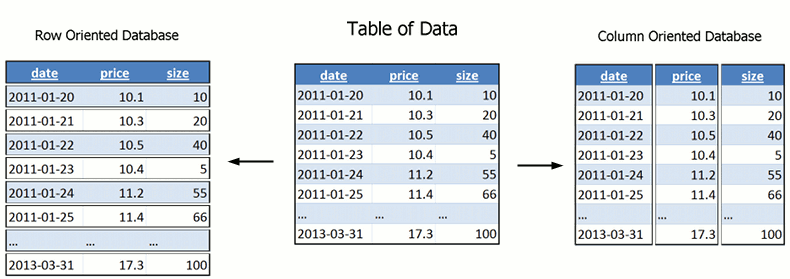
\includegraphics[width=0.8\textwidth]{column-vs-row-oriented-database.png}
	    \caption{Αποθήκευση κατά Σειρές και κατά Στήλες.}
	    \label{fig:column-oriented-dbs}
	\end{figure}
	
	Ένα σημαντικό χαρακτηριστικό που έχουν τέτοια συστήματα είναι οι ενσωματωμένες δυνατότητες για συμπίεση των δεδομένων, αφού η οργάνωση κατά στήλες κάνει τα δεδομένα που βρίσκονται σε μία στήλη να είναι όμοια και έτσι οι αλγόριθμοι συμπίεσης πετυχαίνουν καλύτερα αποτελέσματα. Το χαρακτηριστικό αυτό γίνεται πολύ σημαντικό όταν ο όγκος των δεδομένων είναι μεγάλος. Είναι γενικά καλό με τις συγκεκριμένες βάσεις να υπάρχει ένα πλάνο για το πώς θα χρησιμοποιηθούν τα δεδομένα και τι ερωτήματα θα γίνονται σε αυτά, έτσι ώστε να γίνει κατάλληλη επιλογή της δομής των δεδομένων και να είναι αποδοτική η βάση στη συνέχεια. Αν δεν είναι δυνατόν να γίνει μία τέτοια εκτίμηση εκ των προτέρων, τότε τα συγκεκριμένα συστήματα μπορεί να μην αναδεικνύουν τα δυνατά τους χαρακτηριστικά. Παραδείγματα τέτοιων συστημάτων βάσεων δεδομένων είναι τα BigTable, Cassandra, Hyperbase και HBase\cite{abadi2006integrating}\cite{abadi2009column}.
	
		\subsubsection{Document-oriented Databases (Βάσεις δεδομένων βασισμένες στα έγγραφα)}
		Οι βάσεις οργανωμένες κατά αρχεία, όπως λέει και το όνομά τους, χρησιμοποιούν αρχεία για να αποθηκεύσουν τα δεδομένα. Τα αρχεία αυτά έχουν ένα μοναδικό αναγνωριστικό ID το καθένα και συνήθως η βάση διατηρεί ευρετήριο (index) ώστε να γίνεται γρήγορα η αναζήτηση και η ανάκτηση τους. Σαν τιμή μπορεί να περιέχουν κάθε είδους δεδομένα με μοναδικό περιορισμό να μπορούν να εκφραστούν σαν αρχείο, γεγονός που παρέχει μεγάλη ευελιξία. Τα αρχεία είναι συνήθως τύπου JSON (JavaScript Object Notation) είτε παραλλαγές όπως BSON (Binary JSON) τα οποία είναι κατάλληλα τόσο για την μεταφορά και την αποθήκευση, όσο και για την ανάγνωση και τον χειρισμό των δεδομένων, αφού είναι ένα πρότυπο με το οποίο τα δεδομένα περιγράφουν από μόνα τους τη δομή τους, χωρίς αυτό να προσθέτει κάποιο περιορισμό στη βάση. Λόγω της φύσης των αρχείων, συνήθως τέτοιου είδους συστήματα ταιριάζουν με αντικειμενοστραφείς γλώσσες προγραμματισμού. Μία ιδιαιτερότητα των βάσεων που οργανώνονται κατά αρχεία είναι ότι τα δεδομένα κατά βάση δεν είναι κανονικοποιημένα όπως στις σχεσιακές βάσεις, αλλά κάθε αρχείο προβλέπεται να διατηρεί τις περισσότερες αν όχι όλες τις πληροφορίες που μπορεί να χρειαστούν όταν πραγματοποιείται η ενέργεια που το αφορά. Παραδείγματα τέτοιων συστημάτων βάσεων δεδομένων είναι τα MongoDB, CouchDB, Couchbase, RethinkDB, Terrastore, Elasticsearch\cite{banker2011mongodb}\cite{redmond2012seven}.
		
	\begin{figure}[h]
	    \centering
	    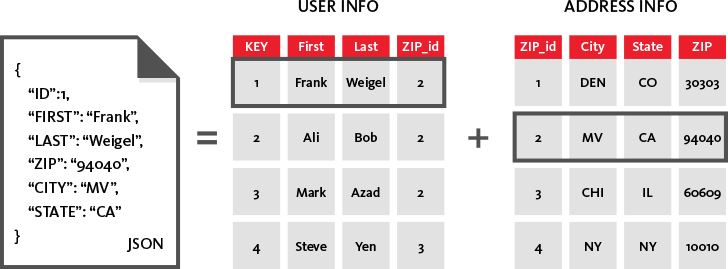
\includegraphics[width=0.7\textwidth]{document_oriented_db.png}
	    \caption{Βάσεις δεδομένων βασισμένες στα έγγραφα.}
	    \label{fig:document_oriented_db}
	\end{figure}
		
		\subsubsection{Graph databases (Βάσεις δεδομένων γράφου)}
		Βασίζονται στη θεωρία των γράφων για την κατασκευή συστημάτων με κόμβους, οι οποίοι τοποθετούνται ανάλογα με τις σχέσεις που προκύπτουν μεταξύ των δεδομένων. Οι βάσεις δεδομένων αυτής της κατηγορίας δεν χρησιμοποιούνται συχνά, αφού είναι κατάλληλη επιλογή μόνο σε περιπτώσεις οπού τα δεδομένα παρουσιάζουν μεγάλη συσχέτιση μεταξύ τους και η συσχέτιση αυτή πρέπει να αποτυπωθεί. Μοντελοποιούνται με κόμβους και με σχέσεις που τους συνδέουν. Χαρακτηριστική λειτουργία σε τέτοιου είδους βάσεις είναι να διασχίζονται οι κόμβοι χρησιμοποιώντας τις σχέσεις που τους συνδέουν. Τέλος, οι κόμβοι και οι σχέσεις μπορούν να έχουν ιδιότητες στις οποίες αποθηκεύονται δεδομένα. Η κλασσική χρήση τέτοιων συστημάτων είναι σε κοινωνικά δίκτυα, όπου οι σχέσεις μεταξύ των χρηστών είναι πολλές και πολύπλοκες. Σε τέτοιες περιπτώσεις τα υπόλοιπα συστήματα βάσεων δεδομένων ταιριάζουν αρκετά λιγότερο και προσθέτουν δυσκολίες. Το γεγονός όμως ότι οι εξαρτήσεις μεταξύ των δεδομένων είναι τόσο πολλές, καθιστά δύσκολο το να γίνουν αυτά τα συστήματα κατανεμημένα, αφού σε περίπτωση κατάτμησης λόγω δικτύου οι σχέσεις που δεν θα είναι πλέον προσβάσιμες μπορεί να είναι πάρα πολλές. Παράδειγμα τέτοιων συστημάτων είναι τα Neo4j, AllegroGraph, GraphDB, FlockDB, OrientDB\cite{he2008graphs}\cite{robinson2013graph}.
		
		\subsubsection{Object-oriented databases (Αντικειμενοστραφείς βάσεις)}
		Οι αντικειμενοστρεφείς βάσεις δεδομένων αποθηκεύουν τα δεδομένα τους, όπως υποδεικνύει το όνομά τους με τη μορφή αντικειμένων, όπως αυτά χρησιμοποιούνται στις αντικειμενοστρεφείς γλώσσες προγραμματισμού. Αυτό κάνει πιο άμεση και απλή τη χρησιμοποίησή τους από εφαρμογές γραμμένες σε τέτοιου είδους γλώσσες, αφού δε χρειάζεται η χρήση επιπλέον κώδικα για την αντιστοίχιση των δεδομένων με την εφαρμογή. Το γεγονός ότι δε χρειάζεται κάποια μετάφραση των αντικειμένων που χρησιμοποιούνται, σε κάποια άλλη μορφή (πχ κατάλληλη για σχεσιακές βάσεις), κάνει τις αντικειμενοστρεφείς βάσεις να παρουσιάζουν συχνά αυξημένη επίδοση σε σχέση με άλλα συστήματα. Επίσης δεν είναι απαραίτητη η δημιουργία κλειδιών για να επιτευχθεί η συσχέτιση και η αντιστοίχιση των δεδομένων, τα οποία μπορούν να αναζητηθούν με τη χρήση δεικτών (pointers).
		
		Οι αντικειμενοστρεφείς βάσεις δεδομένων έχουν εμφανιστεί από τα μέσα της δεκαετίας του 70 και βρήκαν ανταπόκριση σε κάποιες εφαρμογές όπως CAD (Computer Aided Design), CAM (Computer Aided Manufacturing) και σε ενσωματωμένα συστήματα, όμως ποτέ δεν έγινε εκτεταμένη χρήση τους. Αυτό οφείλεται σε κάποια μειονεκτήματα που παρουσιάζουν σε σχέση με άλλα συστήματα. Το κυριότερο από αυτά είναι ότι η βάση που δημιουργείται συσχετίζεται στενά με την εφαρμογή που τη χρησιμοποιεί και πιθανώς και με τη γλώσσα στην οποία είναι γραμμένη η εφαρμογή. Αυτό κάνει τη βάση λιγότερο ευέλικτη σε σχέση με άλλες εναλλακτικές. Επίσης για απλές περιπτώσεις βάσεων που περιέχουν απλές σχέσεις, οι αντικειμενοστρεφείς βάσεις μπορεί να είναι λιγότερο αποδοτικές και πιο πολύπλοκες σε σχέση με ένα σύστημα RDBMS. Παράδειγμα τέτοιων συστημάτων είναι τα VelocityDB, Versand, Objectivity, Starcounter, Perst, HSS Database, Sterling\cite{bertino1997object}\cite{kim1990introduction}\cite{kim2014object}\cite{leavitt2000whatever}.
		
		\subsubsection{Χαρακτηριστικά NoSQL βάσεων δεδομένων}
		
		\subsubsection{Ανθεκτικότητα}
		Όπως και στις σχεσιακές βάσεις, έτσι και στις NoSQL βάσεις όταν κάτι γραφτεί στο δίσκο είμαστε σίγουροι πως δε θα χαθεί. Η διαφορά από τις σχεσιακές βάσεις βέβαια είναι πως στα κατανεμημένα συστήματα κάτι τέτοιο σημαίνει πως η πληροφορία έχει γραφτεί εκ προεπιλογής σε παραπάνω από έναν δίσκο και επομένως δε θα χαθεί ακόμα και σε περίπτωση αποτυχίας ενός δίσκου ή υπολογιστή\cite{schindler2012characteristics}\cite{stonebraker2010sql}.
		
		\subsubsection{Προσαρμοστικότητα}
		Οι NoSQL βάσεις είναι ευέλικτες σχετικά με τα δεδομένα που αποθηκεύουν. Δεν υπάρχει περιορισμός στον τύπο των δεδομένων που μπορούν να αποθηκευτούν, ενώ στις SQL βάσεις ο τύπος έχει καθοριστεί κατά τη δημιουργία τους. Ακόμη, οι NoSQL βάσεις μπορούν να αντιμετωπίσουν με ευκολία πιο πολύπλοκες και προηγμένες δομές δεδομένων. Οι περισσότερες από τις υπάρχουσες NoSQL βάσεις, παρέχουν πλούσιες δομές δεδομένων και εργασιών σε λίστες, σύνολα, ταξινομημένα σύνολα και κλειδιά κατακερματισμού που κάνουν πράγματα όπως εξισορρόπηση φορτίου και message-queuing απλούστατα στην υλοποίηση\cite{stonebraker2010sql}\cite{grazioli2014mapping}.
		
		\subsubsection{Διαχειρισιμότητα}
		Η ύπαρξη ενός άριστα εκπαιδευμένου, με πολλή εμπειρία και γνώση, διαχειριστή βάσεων δεδομένων είναι απαραίτητη για τη συντήρηση ενός υψηλού επιπέδου RDBMS. Είναι άρρηκτα συνδεδεμένος με όλες τις λειτουργίες που αφορούν τη βάση, δηλαδή με το σχεδιασμό, την εγκατάσταση και τη συνεχή παρακολούθηση και ρύθμιση της. Οι μη σχεσιακές βάσεις από τα θεμέλιά τους έχουν σχεδιαστεί για να χρειάζονται λιγότερη διαχείριση. Η δυνατότητα αυτόματης επισκευής, η διανομή δεδομένων, το απλούστερο μοντέλο δεδομένων είναι όλα χαρακτηριστικά που συντελούν στη μείωση των απαιτήσεων σε θέματα ρύθμισης και διαχείρισης\cite{stonebraker2010sql}.
		
		\subsubsection{Παράλληλη επεξεργασία}
		Χάρη στις δυνατότητες που προσφέρουν τα συστήματα NoSQL, όπως εύκολη αναπαραγωγή και διαμοιρασμός δεδομένων, καθίσταται εξίσου εύκολη και η εκμετάλλευση των φυσικών πόρων του συμπλέγματος όπου λειτουργεί η βάση. Από τη στιγμή που τα δεδομένα βρίσκονται σε διαφορετικούς δίσκους, υπολογιστές ή ακόμα και δίκτυα, τα ερωτήματα μπορούν χωρίς καθόλου επιπλέον κώδικα να εκτελούνται παράλληλα και να δίνουν άμεσα απαντήσεις\cite{stonebraker2010sql}.
		
		\subsubsection{Διαθεσιμότητα}
		Όπως θα ήταν αναμενόμενο, δε συμφέρει καθόλου κάποια web ή mobile based επιχείρηση (π.χ. facebook) να είναι πεσμένη. Θέλει δηλαδή να υπάρχει όσο το δυνατόν λιγότερο downtime. Χάρη πάλι στο γεγονός ότι οι NoSQL βάσεις είναι κατανεμημένες, οι ενημερώσεις λογισμικού, αναβαθμίσεις υλικού αλλά και τυχόν αποτυχίες υλικού δε σημαίνουν πως θα πέσει η εφαρμογή, αφού υπάρχει σε πολλαπλούς servers. Αντιθέτως, αν η εφαρμογή βασίζεται σε μία σχεσιακή βάση, τα παραπάνω ισοδυναμούν με δυσκολίες και downtime\cite{stonebraker2010sql}.
		
		\subsubsection{Υψηλή απόδοση}
		Εκτός από το γεγονός ότι με την προσθήκη υπολογιστών στο cluster έχουμε ήδη περισσότερη υπολογιστική ισχύ και άρα καλύτερη απόδοση, η ίδια η αρχιτεκτονική των NoSQL εργαλείων κάνει τις βάσεις αυτές πιο αποδοτικές. Αν μία σχεσιακή βάση είχε μερικές εκατοντάδες χιλιάδες πίνακες, η επεξεργασία των δεδομένων θα δημιουργούσε πάρα πολλά locks και θα υποβάθμιζε την απόδοση. Λόγω όμως της ασθενέστερης συνέπειας που χαρακτηρίζει τα μοντέλα δεδομένων των NoSQL βάσεων, δίνεται βάρος στην αποτελεσματικότητα αντί της συνοχής και επομένως δεν υπάρχει πρόβλημα όσο μεγάλη και να είναι η βάση\cite{stonebraker2010sql}.
		
		\subsubsection{Αναπαραγωγή δεδομένων}
		Τα δεδομένα διανέμονται μεταξύ πολλών κόμβων με πολύ εύκολο τρόπο. Σε όλα τα NoSQL συστήματα κάτι τέτοιο ρυθμίζεται πολύ απλά βάζοντας σε ένα .conf αρχείο την ip ή το domain name των servers στους οποίους θέλουμε να αναπαράγονται τα δεδομένα. Η αυτοματοποίηση της αναπαραγωγής έχει ως αποτέλεσμα την υψηλή διαθεσιμότητα των δεδομένων και επομένως την εύκολη αποκατάσταση από καταστροφή τους, χωρίς να εμπλέκονται ξεχωριστές εφαρμογές για το σκοπό αυτό. Ακόμη, χάρη σε αυτό το χαρακτηριστικό, η προσθήκη ή αφαίρεση υλικού (υπολογιστές, servers κλπ) γίνεται χωρίς downtime\cite{stonebraker2010sql}.
		
		\subsubsection{Schema-less persistence – Δυναμικά Schemas}
		Στις σχεσιακές βάσεις είναι απαραίτητο το σχήμα να είναι ορισμένο πριν αρχίσουμε να προσθέτουμε δεδομένα. Για παράδειγμα, αν θέλουμε να κρατάμε σε κάποια SQL βάση  90 δεδομένα όπως όνομα, επώνυμο και τηλέφωνο πελάτη, είναι απαραίτητο η βάση αυτή να το γνωρίζει από πριν.
		
		Τώρα όμως που ο ρυθμός αύξησης των δυνατοτήτων ιστοσελίδων/εφαρμογών είναι ταχύτατος, κάθε φορά που ολοκληρώνεται κάποιο νέο χαρακτηριστικό, είναι πολύ πιθανό να χρειάζεται αλλαγή και το σχήμα της βάσης. Αν θέλω δηλαδή στη βάση του παραδείγματος να ξεκινήσω να κρατάω και κάτι παραπάνω για τους πελάτες, πρέπει να αλλάξω το σχήμα και να προσθέσω στήλη και ίσως να φτιάξω επιπλέον indexes/foreign keys κλπ. Αν η βάση είναι μεγάλη, η διαδικασία αυτή θα πάρει πολλή ώρα οπότε η βάση δε θα λειτουργεί για το διάστημα αυτό. Επίσης, με ένα σχεσιακό σύστημα, δεν υπάρχει τρόπος να αντιμετωπίσουμε δεδομένα που είναι αδόμητα ή άγνωστα από πριν. Επομένως, το φλέγον θέμα της διαχείρισης των αλλαγών (change management) είναι μεγάλος πονοκέφαλος σε ένα μεγάλο RDBMS.
		
		Αντιθέτως, οι NoSQL βάσεις είναι πολύ ευέλικτες και έχουν χαλαρούς (ή και ανύπαρκτους) περιορισμούς όσον αφορά στο μοντέλο δεδομένων. Είναι σχεδιασμένες να επιτρέπουν την εισαγωγή δεδομένων χωρίς την ύπαρξη προκαθορισμένου σχήματος. Έτσι, οι σημαντικές αλλαγές που χρειάζονται γίνονται σε πραγματικό χρόνο, χωρίς την ανησυχία για διακοπή της λειτουργίας της βάσης. Επομένως, η ανάπτυξη καθίσταται γρηγορότερη, η ενσωμάτωση κώδικα πιο αξιόπιστη και χρειάζεται λιγότερη ώρα ενασχόλησης του διαχειριστή της βάσης\cite{stonebraker2010sql}.
		
		\subsubsection{Κλιμάκωση}
		Είναι ίσως το πιο σημαντικό χαρακτηριστικό των NoSQL βάσεων. Όταν οι επισκέψεις σε ένα site γίνονται μερικές εκατοντάδες ή και χιλιάδες το δευτερόλεπτο, μία σχεσιακή βάση θα έπρεπε να είναι διαμοιρασμένη και αναπαραγμένη σε μεγάλο βαθμό για να καταφέρει να ανταποκριθεί. Μία NoSQL βάση όμως, λόγω της κατανεμημένης της φύσης, το μόνο που χρειάζεται για σωστή κλιμάκωση, είναι προσθήκη υπολογιστών στο σύμπλεγμα (cluster). Δε χρειάζεται ούτε σπατάλη του χρόνου του διαχειριστή της βάσης, ούτε πολύπλοκος κώδικας για partitioning και replication. Ιδιαίτερα με τις νέες τεχνολογίες του cloud και των virtual machines, η κλιμάκωση είναι ιδιαίτερα εύκολη και φθηνή λύση\cite{stonebraker2010sql}. Σε αυτό το σημείο θα πρέπει να αναφερθεί ότι για την κλιμάκωση μιας βάσης δεδομένων υπάρχουν δύο επιλογές α)κατακόρυφη, β)οριζόντια κλιμάκωση. Κατακόρυφη σημαίνει να αυξάνονται συνεχώς οι δυνατότητες των υπαρχόντων εξυπηρετητών ενώ οριζόντια σημαίνει απλά προσθήκη υπολογιστών στο σύμπλεγμα όπως αναφέρθηκε και παραπάνω.
		
		\begin{itemize}
			\item {\textbf{Κατακόρυφη κλιμάκωση}}\\
			Στο επίπεδο της εφαρμογής της αρχιτεκτονικής διαδικτύου τριών επιπέδων, η οριζόντια κλιμάκωση ήταν η προεπιλεγμένη λύση για πολλά χρόνια και λειτουργούσε πολύ καλά. Καθώς όλο και περισσότεροι άνθρωποι χρησιμοποιούν μια εφαρμογή, περισσότεροι εξυπηρετητές του εμπορίου προστίθενται στο επίπεδο της εφαρμογής, η απόδοση διατηρείται με την κατανομή του φόρτου εργασίας σε ένα αυξημένο αριθμό εξυπηρετητών και το κόστος κλιμακώνεται γραμμικά σε σχέση με τον αριθμό των χρηστών
			
	\begin{figure}[h]
	    \centering
	    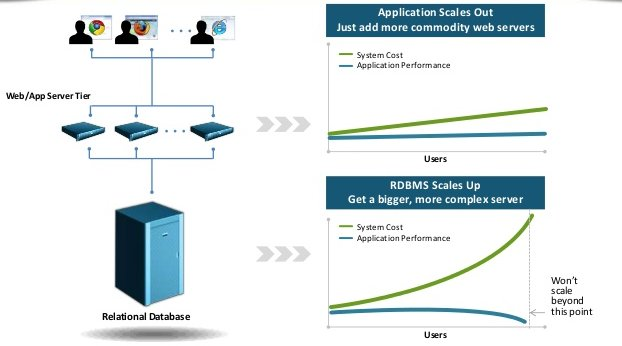
\includegraphics[width=1\textwidth]{RDBMS_scales_up.jpg}
	    \caption{Κλιμακωσιμότητα RDBMS.}
	    \label{fig:RDBMS_scales_up}
	\end{figure}	
			
			Πριν από τις NoSQL βάσεις δεδομένων, η προεπιλεγμένη προσέγγιση ως προς την κλιμάκωση στο επίπεδο της βάσης δεδομένων ήταν η κατακόρυφη κλιμάκωση. Αυτό υπαγορευόταν από τη θεμελιωδώς συγκεντρωτική αρχιτεκτονική της σχεσιακής τεχνολογίας βάσεων δεδομένων. Για την υποστήριξη περισσότερων ταυτόχρονων χρηστών και/ή την αποθήκευση περισσότερων δεδομένων, χρειάζονται όλο και υψηλότερων δυνατοτήτων εξυπηρετητές με περισσότερους επεξεργαστές, περισσότερη μνήμη και περισσότερο αποθηκευτικό χώρο για όλους τους πίνακες. Οι μεγάλοι εξυπηρετητές τείνουν να είναι πολύ πολύπλοκοι, ιδιοταγείς και δυσανάλογα ακριβοί εν αντιθέσει με αυτούς του εμπορίου.	
				
		\item {\textbf{Οριζόντια κλιμάκωση}}\\		
		Οι NoSQL βάσεις δεδομένων αναπτύχθηκαν εξ αρχής ώστε να είναι κατανεμημένες και να ευνοούν την οριζόντια κλιμάκωση. Χρησιμοποιούν ένα σύμπλεγμα τυπικών, φυσικών ή εικονικών εξυπηρετητών για να αποθηκεύουν δεδομένα και να υποστηρίζουν τις λειτουργίες της βάσης δεδομένων. Για κλιμάκωση, επιπλέον εξυπηρετητές προστίθενται στο σύμπλεγμα και τα δεδομένα και οι λειτουργίες της βάσης δεδομένων μοιράζονται στο μεγαλύτερο σύμπλεγμα. Επίσης, επειδή οι εξυπηρετητές του εμπορίου αναμένεται να παρουσιάσουν σφάλματα ανά κάποια χρονικά διαστήματα, οι βάσεις δεδομένων NoSQL έχουν δημιουργηθεί έτσι ώστε να είναι ανεκτικές και να ανακάμπτουν από τέτοια προβλήματα και αυτό τις καθιστά πολύ ανθεκτικές. Οι NoSQL βάσεις δεδομένων παρέχουν μια πολύ ευκολότερη και γραμμική προσέγγιση στην κλιμάκωση των βάσεων δεδομένων. Για κάθε 10,000 νέους χρήστες που αρχίζουν να χρησιμοποιούν μια εφαρμογή, τότε πρέπει απλά να προστεθεί μια ένας νέος εξυπηρετητής βάσης δεδομένων στο σύμπλεγμα. Με αυτόν τον τρόπο η εφαρμογή δεν χρειάζεται τροποποίηση καθώς αυτή βλέπει συνέχεια μόνο μια (κατανεμημένη) βάση δεδομένων.
		
	\begin{figure}[h]
	    \centering
	    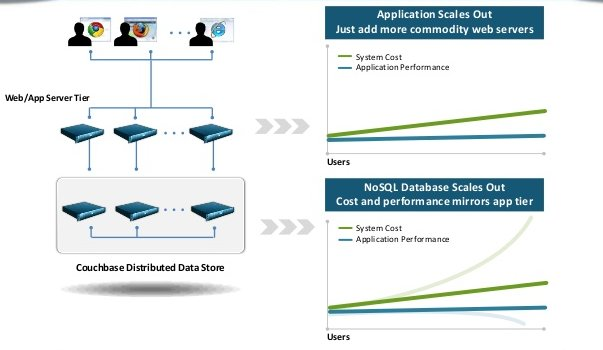
\includegraphics[width=1\textwidth]{nosql_scales_out.jpg}
	    \caption{Κλιμακωσιμότητα NoSQL.}
	    \label{fig:nosql_scales_out}
	\end{figure}
	
	Μια κατανεμημένη προσέγγιση οριζόντιας κλιμάκωσης επίσης συνήθως καταλήγει να είναι φθηνότερη από την εναλλακτική κατακόρυφης κλιμάκωσης. Αυτό είναι συνέπεια του ότι οι μεγάλοι, πολύπλοκοι και ανεκτικοί στα σφάλματα εξυπηρετητές έχουν υψηλά κόστη σχεδιασμού, κατασκευής και συντήρησης. Τα κόστη των αδειών των εμπορικών σχεσιακών βάσεων δεδομένων μπορεί επίσης να είναι απαγορευτικά, λόγω του ότι κοστολογούνται θεωρώντας ότι θα χρησιμοποιηθεί ένας μόνο εξυπηρετητής. Από την άλλη, οι βάσεις δεδομένων NoSQL είναι γενικά ανοιχτού κώδικα και κοστολογούνται με βάση το ότι θα χρησιμοποιηθούν σε ένα σύμπλεγμα εξυπηρετητών και είναι περισσότερο οικονομικές.		
		
		\end{itemize}
		
		\subsubsection{Ενσωματωμένο caching}
		Οι περισσότερες NoSQL βάσεις παρέχουν τεχνολογίες ενσωματωμένου caching. Τα συχνά χρησιμοποιούμενα δεδομένα αποθηκεύονται στη μνήμη όσο το δυνατόν περισσότερο και επομένως η επικοινωνία με το δίσκο ελαχιστοποιείται. Έτσι δεν υπάρχει η ανάγκη για ξεχωριστό επίπεδο caching, ενώ στις περισσότερες SQL βάσεις χρειάζεται ξεχωριστή υποδομή για να επιτευχθεί κάτι τέτοιο\cite{stonebraker2010sql}.
		
		\subsubsection{Μικρότερο κόστος}
		Στις NoSQL βάσεις χρησιμοποιούνται φθηνοί, απλοί servers που μπορεί να βρίσκονται και στο cloud ή να είναι εικονικοί. Από την άλλη, τα RDBMS βασίζονται σε ακριβούς, ιδιωτικούς servers και συστήματα αποθήκευσης. Το κόστος gb ή δοσοληψία ανά δευτερόλεπτο είναι επομένως πολύ χαμηλότερο σε ένα σύστημα NoSQL από ένα σύστημα SQL\cite{stonebraker2010sql}.
\section{Front-End}
	\subsection{Αρχιτεκτονική}
		\subsubsection{MVC αρχιτεκτονικό πρότυπο}\label{sssection:mvc}

		Το σχεδιαστικό μοτίβο Model View Controller (MVC) είναι ένα αρχιτεκτονικό πρότυπο που χρησιμοποιείται στην τεχνολογία λογισμικού και συνήθως στην υλοποίηση web εφαρμογών. Χωρίζει την εφαρμογή σε τρία διασυνδεδεμένα μέρη, με σκοπό τον πλήρη διαχωρισμό της εσωτερικής αναπαράστασης της πληροφορίας στο σύστημα από τους τρόπους παρουσίασης της πληροφορίας στον χρήστη. Το MVC αποτελείται από τρία στοιχεία: α) Model, β) View, γ) Controller.
		\begin{itemize} 
		\item\textbf{Model:} Το model είναι το κομμάτι της εφαρμογής που αναπαριστά την πληροφορία, δηλαδή τα δεδομένα που χρησιμοποιεί η εφαρμογή και επιβάλλει τις ενέργειες και τους περιορισμούς πάνω σε αυτά.  Στο model τοποθετούμε τις λειτουργίες της εφαρμογής που σχετίζονται με την πρόσβαση στη βάση δεδομένων. Οι λειτουργίες αυτές είναι συναρτήσεις με τις οποίες διαχειριζόμαστε αποτελεσματικά τα δεδομένα που λαμβάνουμε από τη βάση.  Το μοντέλο ανταποκρίνεται σε ερωτήματα από το view καθώς και σε οδηγίες από τον controller για να πραγματοποιήσει ενημερώσεις.
		\item\textbf{View:} Αντιστοιχεί στη γραφική παρουσίαση των δεδομένων του model στο interface του χρήστη. Ο controller, είναι αυτός ο οποίος αποφασίζει πότε θα παρουσιαστούν τα δεδομένα ενώ το view καθορίζει τον τρόπο με τον οποίο θα παρουσιαστούν τα δεδομένα στον χρήστη. Το επίπεδο view θα πρέπει να προσαρμόζεται στις αλλαγές του επιπέδου του model, για αυτό και τα views θα πρέπει να επικεντρώνονται μόνο στην εμφάνιση δεδομένων και να μην εμπλέκονται με την επιχειρηματική λογική του model.
		\item\textbf{Controller:} Ο controller είναι αυτός που παίρνει αποφάσεις, δηλαδή διαχειρίζεται τη σύνδεση των δεδομένων του model με τη λογική του προγράμματος και καθορίζει ποια από τα δεδομένα του model θα παρουσιαστούν από το view στο interface του χρήστη. Ο controller ενημερώνει το view κάθε φορά που αλλάζει το model. Επιπλέον προσθέτει event listeners στο view και ενημερώνει το model όταν ο χρήστης αλληλεπιδρά με το view.
	 \end{itemize}		
	 \begin{figure}[h]
	    \centering
	    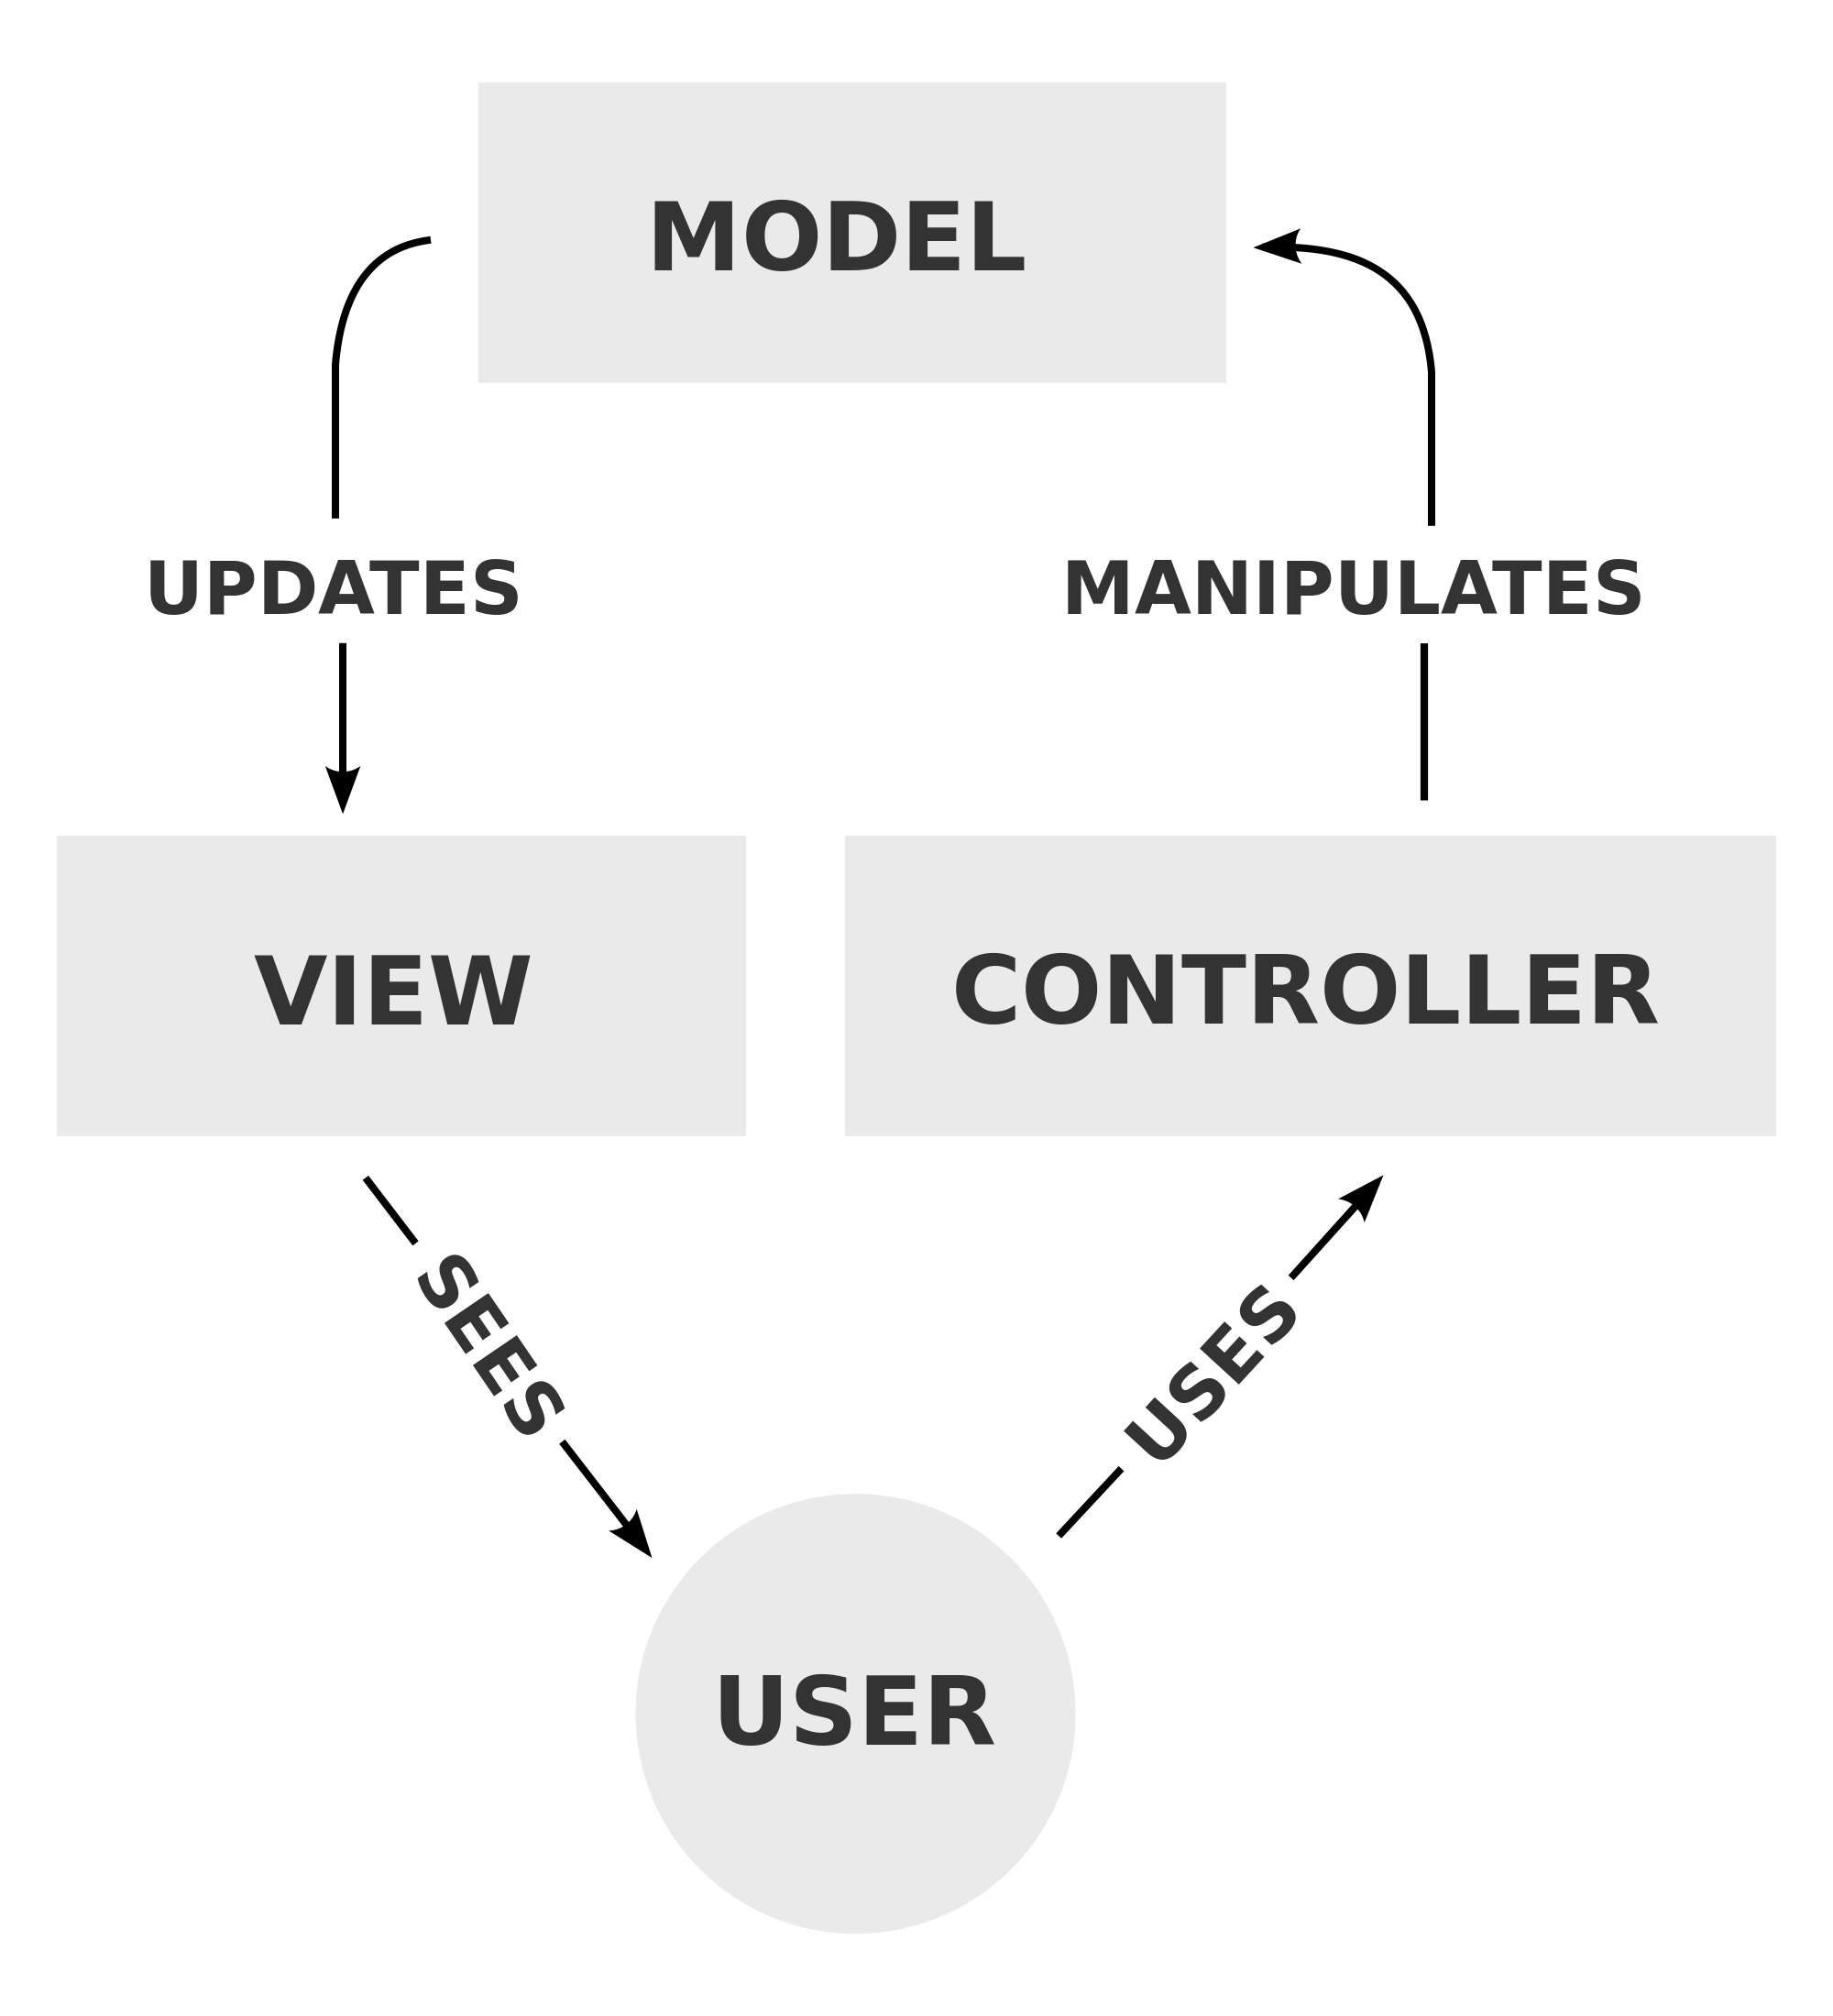
\includegraphics[width=0.7\textwidth]{mvcpattern.png}
	    \caption{Αρχιτεκτονική MVC.}
	    \label{fig:mvc_pattern}
	\end{figure}
		
		
		Η  χρήση της αρχιτεκτονικής MVC κατά την δημιουργία μίας εφαρμογής μας προσφέρει τα εξής βασικά πλεονεκτήματα:
		\begin{itemize}
		\item Διαχωρισμός των προβλημάτων (Separation of Concerns). Ουσιαστικά δημιουργείται μία εφαρμογή η οποία έχει τρία επίπεδα(models, views, controllers) και το κάθε επίπεδο επιτελεί ξεχωριστό έργο και ταυτόχρονα συνεργάζεται με τα άλλα επίπεδα. Στην σωστή υλοποίηση πρέπει τα τρία επίπεδα να είναι πλήρως καθορισμένα και να μην συμπλέκονται. Ο διαχωρισμός αυτός, επιτρέπει την επαναχρησιμοποίηση της επιχειρηματικής λογικής σε διάφορες εφαρμογές και την ανάπτυξη πολλαπλών user interfaces χωρίς να προβληματιζόμαστε από τον κώδικα που διαχειρίζεται την βάση.
		\item \textbf{Επεκτασιμότητα (Scaleability)}. Είναι η δυνατότητα που διαθέτει μία εφαρμογή , να μπορούμε μελλοντικά να προσθέσουμε λειτουργίες σε αυτή ή να αλλάξουμε κάποιες από τις ήδη υπάρχουσες λειτουργίες με σκοπό να επιτύχουμε διαφορετικά αποτελέσματα. 
		\item \textbf{Ελεγξιμότητα (Testability)}. Οι MVC εφαρμογές έχουν τη δυνατότητα να είναι πιο εύκολα ελέγξιμες και με τον τρόπο αυτόν συντηρούνται πιο εύκολα.  Εφόσον τα συστατικά της αρχιτεκτονικής είναι διακριτά, είναι πιο εύκολο να γράφουμε κώδικα που να τεστάρει ξεχωριστά το κάθε κομμάτι, γρήγορα και αποτελεσματικά.
		\item \textbf{Παράλληλη ανάπτυξη από διαφορετικές ομάδες}. Οι προγραμματιστές επιχειρηματικής λογικής  μπορούν να δημιουργούν τις κλάσεις, ενώ οι προγραμματιστές του user interface μπορούν να σχεδιάζουν ταυτόχρονα τις οθόνες. Επίσης μπορούν να γίνονται ενημερώσεις και αλλαγές στο user interface χωρίς να επιβραδύνεται η διαδικασία του business logic.
		\end{itemize}
		
	\subsubsection{MVP αρχιτεκτονικό πρότυπο}\label{sssect:MVP_architecture}
	Το αρχιτεκτονικό πρότυπο Model View Presenter (MVP) αποτελεί ένα παράγωγο αρχιτεκτονικό πρότυπο του MVC \cite{mvpPotel}, το οποίο είναι πολύ δημοφιλές στην ανάπτυξη εφαρμογών για το λειτουργικό σύστημα Android. Στην θεωρία τουλάχιστον, οι εφαρμογές Android είναι στημένες με τη λογική του MVC \cite{androidArchAnalysis}, όπως περιγράφηκε στην ενότητα \ref{sssection:mvc}, με το Activity ή το Fragment να αποτελεί τον controller και τα xml layouts τα views. Στην πράξη όμως καταλήγει η πλειονότητα του view logic να βρίσκεται στο Activity το οποίο το μετατρέπει σε δομή model-view όπως φαίνεται στο σχήμα \ref{fig:model_view}, κάτι το οποίο σε καμία περίπτωση δεν είναι το επιθυμητό. Στόχος λοιπόν του MVP είναι να λύσει ακριβώς αυτό το πρόβλημα και να πετύχει πλήρη διαχωρισμό μεταξύ του view και του view logic όπως βλέπουμε στο σχήμα \ref{fig:mvp_pattern}.
		
	 \begin{figure}[h]
	    \centering
	    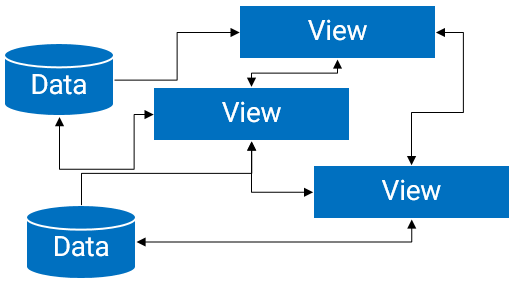
\includegraphics[width=0.7\textwidth]{model_view.png}
	    \caption{Android Model-View αρχιτεκτονικό πρότυπο.}
	    \label{fig:model_view}
	\end{figure}
	
	\begin{figure}[h]
	    \centering
	    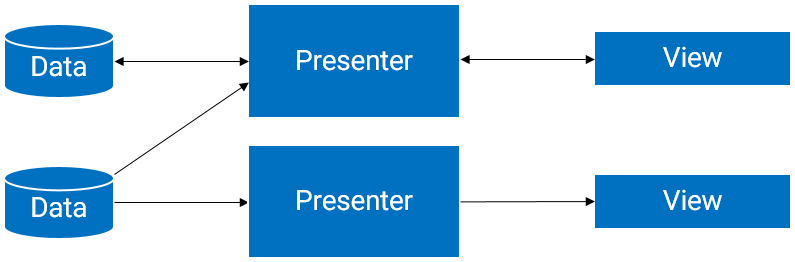
\includegraphics[width=0.7\textwidth]{mvp_pattern.png}
	    \caption{Android MVP αρχιτεκτονικό πρότυπο.}
	    \label{fig:mvp_pattern}
	\end{figure}
	
	Πλεονεκτήματα και λόγοι χρήσης του αρχιτεκτονικού προτύπου Model View Presenter\cite{androidHacks}:
	\begin{itemize}
		\item \textbf{Επεκτασιμότητα} η οποία επιτυγχάνεται μέσω του πλήρη διαχωρισμού μεταξύ της εμφάνισης (view) και της λογικής της εμφάνισης (view logic). 
		\item \textbf{Ευκολία Testing} του κάθε στρώματος (layer) της εφαρμογής αφού έχουμε πετύχει σαφή διαχωρισμό μεταξύ τους. Εν γένει η χρήση του μοτίβου MVP προάγει το test driven development της εφαρμογής με όλα τα πλεονεκτήματα που συνεπάγεται η εν λόγω τεχνική ανάπτυξης.
	\end{itemize}
	
	Το αρχιτεκτονικό πρότυπο MVP όπως δηλώνει και το όνομα του αποτελείται από τα παρακάτω τρία στοιχεία α) Model β) View γ) Presenter :
	\begin{itemize}
		\item \textbf{Model: } Το model στο αρχιτεκτονικό πρότυπο MVP επιτελεί της ίδιες λειτουργίες με αυτές στο MVC όπως περιγράφηκαν παραπάνω στην ενότητα \ref{sssection:mvc}.
		\item \textbf{View: } Το view υλοποιείται συνήθως μέσω κάποιου Activity ή Fragment (εξαρτάται από τη συγκεκριμένη αρχιτεκτονική της εφαρμογής), και περιέχει αναφορά στον presenter ο οποίος το χειρίζεται. H εν λόγω αναφορά πραγματοποιείται με χρήση του σχεδιαστικού μοτίβου dependency injection και ιδανικά με χρήση του Dagger. Κάθε φορά που ο χρήστης αλληλεπιδρά με κάποια λειτουργία (π.χ κουμπί) του view, καλείται η αντίστοιχη συνάρτηση του presenter ο οποίος επικοινωνεί με το model και λέει εν τέλει στο view τι θα εμφανίσει.
		\item \textbf{Presenter: } Ο Presenter είναι λειτουργεί ως το ενδιάμεσο στάδιο - ενορχηστρωτής μεταξύ του view και του model. Είναι υπεύθυνος για την απόκτηση των δεδομένων από το model και την παρουσίαση τους στο view, αλλά σε αντίθεση με την κλασσική αρχιτεκτονική MVC είναι υπεύθυνος για τις αλλαγές που γίνονται στο view όταν ο χρήστης αλληλεπιδρά μαζί του.
	\end{itemize}
	
	Για να αποσαφηνιστεί πλήρως η λειτουργία του και να γίνει πιο εύκολα κατανοητό στο σχήμα \ref{fig:mvp_workflow} βλέπουμε ένα χαρακτηριστικό παράδειγμα.
	
	\begin{figure}[h]
	    \centering
	    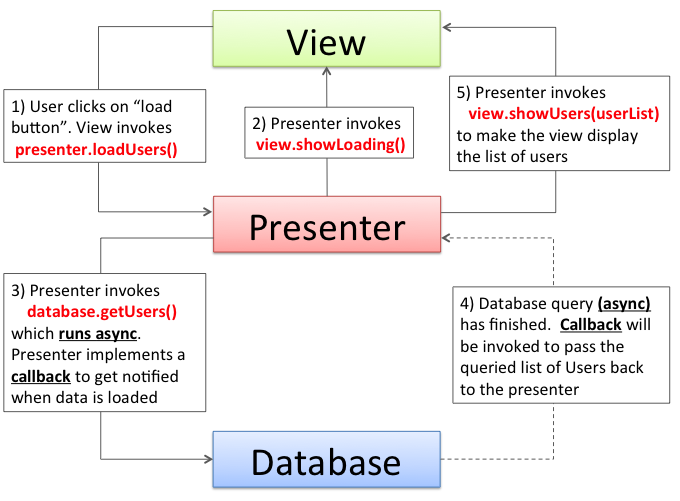
\includegraphics[width=0.7\textwidth]{mvp_workflow.png}
	    \caption{Παράδειγμα MVP σε Android.}
	    \label{fig:mvp_workflow}
	\end{figure}

	\subsection{Frameworks}
	
		Το framework, στον προγραμματισμό ηλεκτρονικών υπολογιστών, είναι μια αφηρημένη έννοια με την οποία κοινός κώδικας ο οποίος παρέχει γενικές λειτουργίες, μπορεί να επανεγγραφεί επιλεκτικά ή να εξειδικευτεί μέσω του κώδικα κάποιου χρήστη ώστε να χρησιμοποιηθεί για συγκεκριμένες λειτουργίες. Τα frameworks είναι μια ειδική περίπτωση βιβλιοθηκών λογισμικού που εμπεριέχουν επαναχρησιμοποιήσιμα κομμάτια κώδικα σε μια καλά καθορισμένη διεπαφή προγραμματισμού εφαρμογών (API), που όμως περιέχουν κάποια βασικά χαρακτηριστικά γνωρίσματα που τα διαφοροποιούν από τις κανονικές βιβλιοθήκες. Κάποια από τα γνωρίσματα αυτά είναι: αντιστροφή του ελέγχου (η ροή του προγράμματος υπαγορεύεται από το framework και όχι από αυτόν που το χρησιμοποιεί), προκαθορισμένη συμπεριφορά, επεκτασιμότητα (μπορεί να επεκταθεί από το χρήστη συνήθως με επανεγγραφή  ή εξειδίκευση του κώδικα ώστε να εκτελούνται συγκεκριμένες λειτουργίες. \cite{Framework}

	
		\subsubsection{Express Framework}


		Το Express είναι ένα δρομολόγησης και middleware framework, το οποίο έχει ελάχιστη λειτουργικότητα από μόνο του. Μια Express εφαρμογή ουσιαστικά αποτελεί μία σειρά από middleware κλήσεις. Ο δημιουργός του Express framework, TJ Holowaychuck, το έχει περιγράψει ως "Sinatra Inspired Server",  που σημαίνει ότι είναι σχετικά ελάχιστο, αλλά παρέχει πολλά επιπλέον χαρακτηριστικά, τα οποία είναι διαθέσιμα ως πρόσθετα. 
		
Το middleware είναι μια συνάρτηση με πρόσβαση στο αντικείμενο της αίτησης (req), το αντικείμενο απάντηση (res), και το επόμενο middleware στον κύκλο αίτησης-απάντησης της εφαρμογής, που συνήθως συμβολίζεται με μια μεταβλητή με το όνομα next.

Το middleware μπορεί να:

\begin{itemize}

\item Εκτελέσει οποιοδήποτε κώδικα.
\item Να κάνει αλλαγές στην αντικείμενα αίτησης και απάντησης(request and response objects).
\item Να τερματίσει τον κύκλο αίτησης-απάντησης.
\item Να καλέσει το επόμενο middleware της στοίβας.
\item Εάν το τρέχον middleware δεν τελειώσει τον κύκλο αίτησης-απάντησης, θα πρέπει να κληθεί το επόμενο, next(), για να περάσει ο έλεγχος στο επόμενο middleware, διαφορετικά η αίτηση θα μείνει ξεκρέμαστη.

\end{itemize}


Μία εφαρμογή Express μπορεί να χρησιμοποιήσει τα ακόλουθα είδη middleware: middleware επιπέδου εφαρμογής (application-level middleware),middleware επιπέδου δρομολόγησης, middleware χειρισμού σφαλμάτων(error-handling middleware), ενσωματωμένο middleware (built-in middleware), middleware τρίτων κατασκευαστών middleware (third-party middleware). 


		\subsubsection{Angular}
		
		Το AngularJS είναι ένα από τα πιο δημοφιλή ανοιχτού κώδικα JavaScript framework που χρησιμοποιείται για την κατασκευή και τη δομή σύγχρονων διαδικτυακών εφαρμογών, κυρίως εφαρμογών μίας σελίδας. Αναπτύχθηκε από τη Google και από μία κοινότητα προγραμματιστών για την αντιμετώπιση των πολλών προκλήσεων που ανέκυψαν κατά την ανάπτυξη των εφαρμογών μίας σελίδας. Στόχος του είναι να απλοποιήσει τόσο την ανάπτυξη όσο και το testing αυτών των εφαρμογών, παρέχοντας ένα framework για client-side model-View-Controller (MVC) και το model-view-viewmodel (MVVM) αρχιτεκτονικές, μαζί με τα συστατικά που χρησιμοποιούνται συνήθως στις εφαρμογές Διαδικτύου.
	   \\*
			    \textbf{Αρχιτεκτονική}
	 \\*
		Κατά την εκκίνηση της εφαρμογής, το πρόγραμμα περιήγησης φορτώνει το HTML αρχείο και το κάνει ``'parse' στο DOM αρχείο, και μαζί με αυτό στο AngularJs script. Μόλις το DOM αρχείο έχει φορτωθεί, το AngularJS αναζητά την εντολή ng-app η οποία ορίζει τα όρια της εφαρμογής. Εάν ορίζεται κάποιο module μέσα στην οδηγία, τότε χρησιμοποιείται για να ρυθμιστεί το \$injector, που δημιουργεί τo \$compile service καθώς και το \$ rootScope. Τότε μεταγλωττίζεται το DOM και συνδέεται στο \$ rootScope μετά από το οποίο εκτελούνται οι υπόλοιπες εντολές (αν υπάρχουν). Στο σχήμα \ref{fig:angularjs} φαίνεται ο κύκλος εκκίνησης του AngularJS.
		
	  \begin{figure}[h]
	    \centering
	    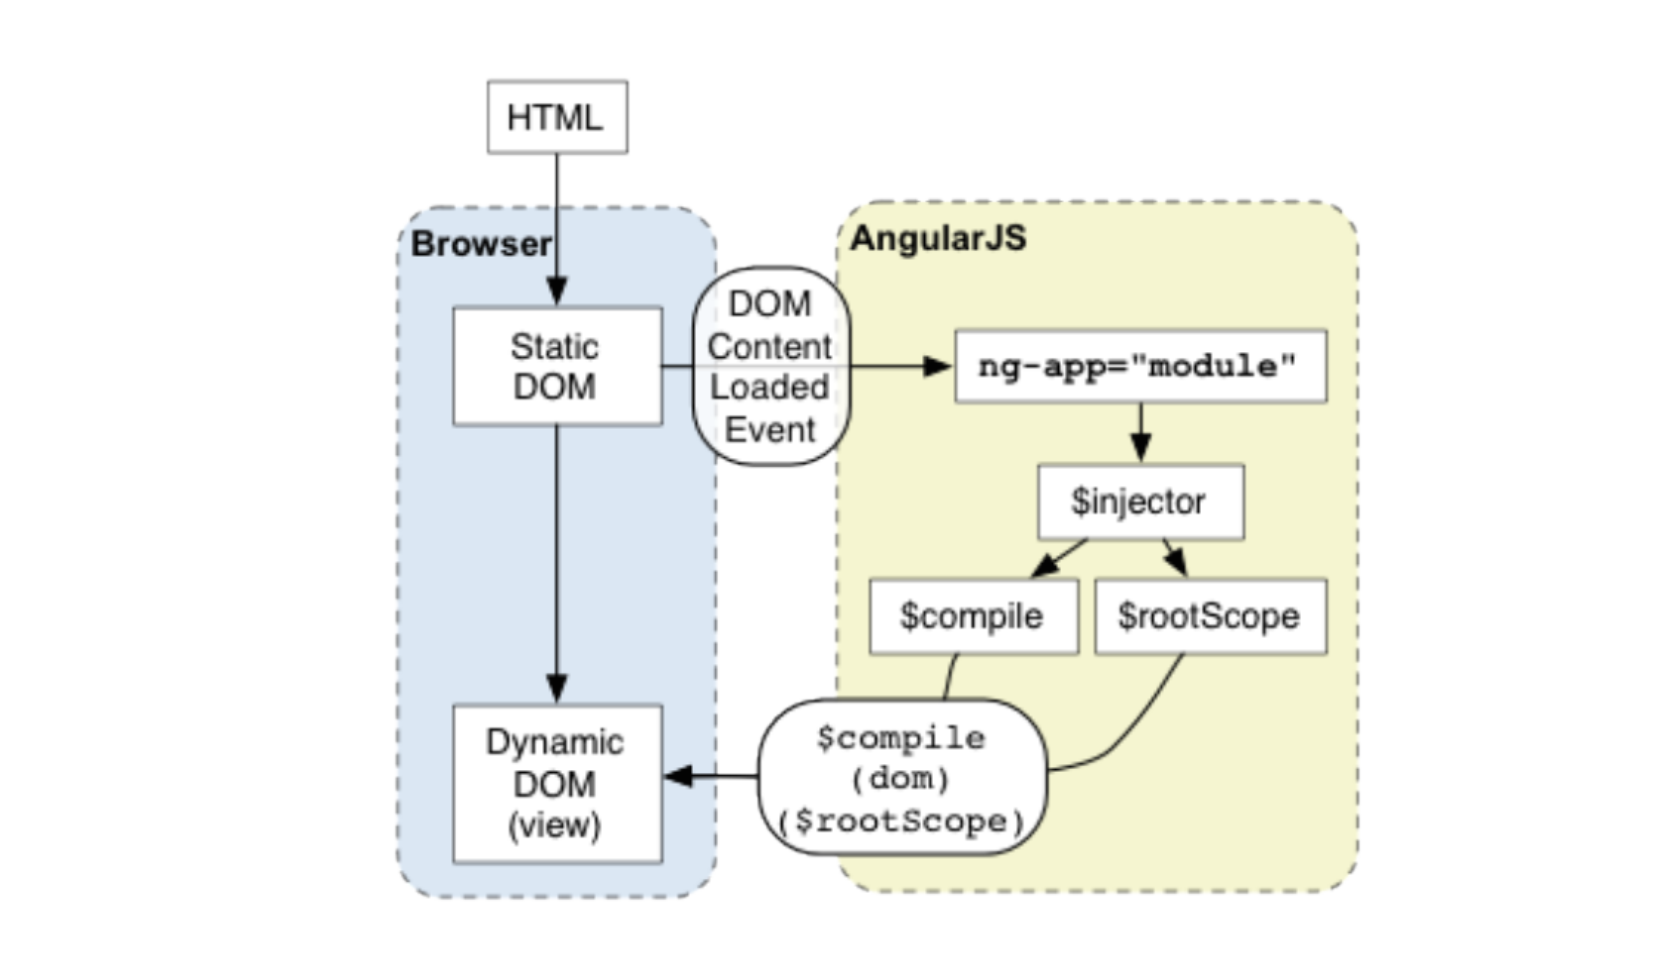
\includegraphics[width=0.7\textwidth]{angularjs.png}
	    \caption{AngularJS κύκλος εκκίνησης.}
	    \label{fig:angularjs}
	\end{figure}

	Κάποια από τα βασικά χαρακτηριστικά του AngularJS είναι:
	\begin{itemize}
	\item Two Way Data-binding. Αυτό πρακτικά σημαίνει ότι όταν αλλάζει το model αλλάζει και το view, και όταν αλλάζει το  view αλλάζει και το model. Το Two Way Data-binding εξηγείται καλύτερα με ένα παράδειγμα: 
	
	
	\lstinputlisting[language=Html]{two_way_data_binding.html}

	Αν ο χρήστης αλλάζει κάποια τιμή του model μέσω της εισόδου στο view, τότε το AngularJs αποθηκεύει την τιμή
αυτή σε μια μεταβλητή. Το στοιχείο h1 στην συνέχεια ενημερώνεται αυτόματα ώστε να αντικατοπτρίζονται οι αλλαγές στην τιμή της μεταβλητής του model. Το view ενημερώνεται ακόμα και αν η μεταβλητή αλλάξει χειροκίνητα με χρήση JavaScript.\cite{angular}

	\item  HTML Templates. Ενώ άλλα JavaScript frameworks χρησιμοποιούν ένα template system που βασίζεται στην HTML με ειδική σήμανση το οποίο μπορεί να είναι δυσκολεύει τους προγραμματιστές, το AngularJS δεν στηρίζεται σε εξωτερικές template engines αλλά χρησιμοποιεί ένα templating σύστημα, που είναι χτισμένη πάνω στην HTML με έξυπνη χρήση των ng- χαρακτηριστικών. Το πρόγραμμα περιήγησης διαβάζει την HTML και ``ψάχνει"  ng - directives τα οποία, όταν εκτελεστούν, δεσμεύουν το view στο model.

    \item Dependency Injection. Το dependency injection ενθαρρύνεται πολύ από το AngularJS και είναι ένα από τα συστατικά του, που βελτιώνει σε μεγάλο βαθμό το testability του. Το dependency injection είναι ένα design pattern λογισμικού στο οποίο σε ένα αντικείμενο ορίζονται οι εξαρτήσεις του και δεν τις δημιουργεί μόνο του. Πρόκειται ουσιαστικά για την αφαίρεση των hard-coded εξαρτήσεων, κάνοντας δυνατό να αλλάξουν οι εξαρτήσεις όποτε χρειαστεί.
      Ένα παράδειγμα είναι όταν υπάρχει μία συνάρτηση η οποία παίρνει μία παράμετρο, όπως:
    	
	\lstinputlisting[language=JavaScript]{angular_dependency_injection.js}

Το παραπάνω παράδειγμα είναι εύκολο να το τεστάρουμε, επειδή το στοιχείο που εισάγεται στην συνάρτηση μπορεί να είναι είτε ένα πραγματικό αντικείμενο ή ένα αντικείμενο για τους σκοπούς των τεστ. Ο διαχωρισμός σε μικρότερα πιο εύκολα ελέγξιμα συστατικά μπορεί να βοηθήσει πολύ στην ανίχνευση των σφαλμάτων.

    \item Deep Linking. Σε μια εφαρμογή μίας σελίδας είναι σημαντικό να διατηρείται η κατάσταση της εφαρμογής στο url, έτσι ώστε οι χρήστες είναι σε θέση να βάλουν κάποιο σελιδοδείκτη ή να μοιραστούν κάποιον σύνδεσμο σε διάφορες καταστάσεις της εφαρμογής.Το AngularJS χρησιμοποιεί το HTML5 history API  μαζί με ένα (\#!) εφεδρικό για παλαιότερα προγράμματα περιήγησης. Η λειτουργία αυτή είναι εξαιρετικά ισχυρή στη σύγχρονη εποχή των κοινωνικών δικτύων και του sharing.

	\item Directives. Τα directives είναι κάτι μοναδικό στο AngularJS και επιτρέπουν την επέκταση της λειτουργικότητας της HTML. Ενώ το AngularJS έχει μια συλλογή από προκαθορισμένα directives, μπορεί να επεκταθεί με συγκεκριμένες λειτουργικότητες σε σημείο που να επιτρέπει στον χρήστη να δημιουργήσει το δικό του DSL (Domain specific language). Επίσης επιτρέπει να δημιουργηθούν προσαρμοσμένα στοιχεία DOM, καθώς και χαρακτηριστικά και κλάσεις στα οποία μπορούν να προστεθούν λειτουργικότητες. Το επόμενο παράδειγμα από το επίσημο documentation του AngularJS δείχνει ότι για παράδειγμα γίνεται να επιτραπούν data-bindings για ένα html στοιχείο, αν υπάρχει ένα συγκεκριμένο χαρακτηριστικό. \cite{angular-directives}
\\*
\textbf{HTML:}

	\lstinputlisting[language=Html]{angular_directives.html}
 
\textbf{JavaScript:}

	\lstinputlisting[language=JavaScript]{angular_directives.js}


	\item \$http service. Το AngularJS είναι εξαιρετικά ευέλικτο στον τρόπο που επικοινωνεί με τα διαφορετικά backends. Αντί να βασίζεται αποκλειστικά στο REST, επικοινωνεί ελεύθερα μέσω των XMLHttpRequests του προγράμματος περιήγησης ή μέσω του JSONP. Παρόλο που το \$ http service προσθέτει http headers ως προεπιλογή στα αιτήματα του,  είναι εύκολα διαμορφώσιμα μέσω του \$httpProvider.defaults.headers.
	\end{itemize}




		\subsubsection{Bootstrap}
	Το bootstrap είναι ένα πάρα πολύ δυνατό front-end framework για την ταχύτερη και ευκολότερη ανάπτυξη ιστοσελίδων. Είναι ουσιαστικά μία συλλογή εργαλείων ανοιχτού κώδικα και περιλαμβάνει HTML και CSS πρότυπα σχεδιασμού για κοινά στοιχεία διεπαφής χρήστη, όπως τυπογραφίας, φόρμες, κουμπιά, πίνακες, dropdowns, alerts, μπάρες, και πολλά άλλα, καθώς και προαιρετικές επεκτάσεις JavaScript. Το bootstrap είναι συμβατό με όλες τις τελευταίες εκδόσεις των προγραμμάτων πλοήγησης και υποστηρίζει "responsive web design". Αυτό σημαίνει πως η διάταξη των ιστοσελίδων προσαρμόζεται δυναμικά, λαμβάνοντας υπόψιν τα χαρακτηριστικά της συσκευής που το χρησιμοποιεί (σταθερός υπολογιστής, κινητό, τάμπλετ κ.τ.λ.). 
	
	Το bootstrap είναι modular και αποτελείται από μικρότερα LESS stylesheets τα οποία υλοποιούν τα διάφορα στοιχεία του πακέτου εργαλείων. Ένα stylesheet, με όνομα bootstrap.less περιλαμβάνει τα επιμέρους stylesheets. Οι προγραμματιστές μπορούν να προσαρμόσουν και οι ίδιοι το bootstrap, καθώς τους δίνεται η δυνατότητα να επιλέξουν τα στοιχεία που θέλουν να χρησιμοποιήσουν. Αναπροσαρμογές γίνονται σε περιορισμένο όμως βαθμό, μέσω ενός κεντρικού stylesheet. Πιο ουσιαστικές αλλαγές πραγματοποιούνται με LESS δηλώσεις. Η χρήση των LESS stylesheets επιτρέπει τη χρήση μεταβλητών, συναρτήσεων καθώς και mixins. Επιπλέον, ο σχεδιαστής μπορεί να επιλέγει σε μια φόρμα τα επιθυμητά στοιχεία και να τα προσαρμόζει, σε τιμές διαφόρων εναλλακτικών λύσεων για τις ανάγκες του. Στη συνέχεια δημιουργείται ένα πακέτο που περιλαμβάνει ήδη το προ-χτισμένο CSS stylesheet.
	
	Το bootstrap παρέχει ένα σύνολο από stylesheets που παρέχουν βασικούς ορισμούς στυλ για όλα τα βασικά HTML στοιχεία. Αυτά παρέχουν ενιαία, σύγχρονη εμφάνιση για πίνακες, μορφοποίηση κειμένου, καθώς και για τα στοιχεία μιας φόρμας. Επιπλέον των HTML στοιχείων, το bootstrap περιέχει και άλλα στοιχεία περιβάλλοντος τα οποία χρησιμοποιούνται συχνά. Αυτά περιλαμβάνουν κουμπιά με προηγμένα χαρακτηριστικά ( π.χ. ομαδοποίηση κουμπιών ή drop-down επιλογή, οριζόντιες και κάθετες καρτέλες, σελιδοποίηση, κ.λ.π. ), ετικέτες, προηγμένες τυπογραφικές δυνατότητες, εικονίδια, προειδοποιητικά μηνύματα και μια γραμμή προόδου. Τέλος, το bootstrap περιέχει πολλά συστατικά JavaScript σε μια μορφή jQuery plugin, τα οποία παρέχουν πρόσθετα στοιχεία διεπαφής χρήστη όπως παράθυρα διαλόγου, επεξηγήσεις, και καρουσέλ. Μπορούν επίσης να επεκτείνουν τη λειτουργικότητα ορισμένων υφιστάμενων στοιχείων της διασύνδεσης, όπως για παράδειγμα μια αυτόματη πλήρη λειτουργία για πεδία εισαγωγής\cite{bootstrap}. 
	Τα πιο σημαντικά πλεονεκτήματα που προκύπτουν από την χρήση του bootstrap είναι:
	\begin{itemize}
	\item \textbf{Ταχύτητα ανάπτυξης: } Αδιαμφισβήτητα, ένα από τα σημαντικότερα πλεονεκτήματα της χρήσης του bootstrap είναι η ταχύτητα της ανάπτυξης. Το bootstrap παρέχει τη δυνατότητα χρήσης έτοιμων μπλοκ κώδικα, έτσι ώστε να γίνεται η αρχή του front-end από εκεί και να μην χρειάζεται να γραφτεί κώδικας από το μηδέν ("from scratch"). Το άνωθεν σε συνδυασμό με τη συμβατότητα σε όλα τα προγράμματα περιήγησης που προσφέρει καθώς και τις λειτουργίες του CSS-LESS, εξοικονομεί πολύτιμο χρόνο στους προγραμματιστές.
	\item \textbf{Ανταποκρισημότητα: } Λόγω του διαρκώς αυξανόμενου αριθμού των κινητών συσκευών υπάρχει η ανάγκη να έχουμε διαδραστικές ιστοσελίδες.Το bootstrap διευκολύνει πάρα πολύ την δημιουργία οθονών για κινητά χάρη στη ρευστή διάταξη πλέγματος που έχει, η οποία προσαρμόζεται δυναμικά στην κατάλληλη ανάλυση οθόνης και δεν χρειάζεται να προβούμε σε επιπλέον ενέργειες για να πετύχουμε την σωστή αποκρισιμότητα.
	\item \textbf{Συνοχή: } Το bootstrap βασίζεται σε αυτή την αρχή καθώς αρχικά αναπτύχθηκε από μερικούς υπαλλήλους του Twitter ως ένα framework για να υπάρχει συνέπεια μεταξύ των εσωτερικών εργαλείων που χρησιμοποιούνταν. Το bootstrap ουσιαστικά χτίστηκε ώστε να "ταιριάζει" τους σχεδιαστές με τους προγραμματιστές και να διασφαλίζει τη συνέπεια, ανεξάρτητα του ποιος εργάζεται στο έργο ή σε ποια πλατφόρμα θα τρέξει.
	\item \textbf{Προσαρμοστικότητα: } Το bootstrap, μπορεί να προσαρμοστεί σύμφωνα με τις προδιαγραφές του κάθε έργου. Οι προγραμματιστές έχουν τη δυνατότητα να επιλέξουν τα χαρακτηριστικά που χρειάζονται και να πετάξουν τα υπόλοιπα.
	\end{itemize}

		
	\subsection{Jade Template Engine}
	

	Μια μηχανή πρότυπο είναι μια βιβλιοθήκη ή ένα framework που χρησιμοποιεί ορισμένους κανόνες ή μία συγκεκριμένη γλώσσα για να ερμηνεύσει τα δεδομένα και να παρουσιάσει τα views. Στην περίπτωση των διαδικτυακών εφαρμογών, τα views είναι σελίδες HTML (ή τμήματα αυτών), αλλά γενικότερα μπορεί να είναι JSON ή XML αρχεία, ή graphic user interfaces. Με βάση το μοντέλο Model-View-Controller (MVC), τα πρότυπα ανήκουν στα views.

		Υπάρχουν πολλοί λόγοι που οδηγούν στη χρήση μιας μηχανή προτύπων αντί για την συγγραφή του front-end κώδικα σε μια συγκεκριμένη γλώσσα. Το μεγάλο πλεονέκτημα αυτής της προσέγγισης, είναι ότι παρουσιάζει HTML στην πλευρά του εξυπηρετητή (server), την οποία στέλνει στον πελάτη (client) και στη συνέχεια όταν ο πελάτης αλληλεπιδράσει με τη σελίδα και η HTML αλλάξει χρησιμοποιώντας τα ίδια bits του πρότυπου και ίσως ακόμη και κάποια κοινή λογική. Άλλοι πολύ σημαντικοί λόγοι αποτελούν η συνέπεια του κώδικα και η οργάνωση.  Εάν υπάρχει καλός διαχωρισμός της σήμανσης (markup) από τη λογική γίνεται πιο εύκολος εντοπισμός σφαλμάτων του κώδικα, κοινή χρήση του κώδικα με συνεργάτες,καθώς και επιτυγχάνεται ταχύτερη ανάπτυξη μέσω της απόκτησης κοινών μεθόδων για την έξοδο της σήμανσης (markup). Οι μηχανές προτύπων που λειτουργούν, εξίσου καλά και από την πλευρά του εξυπηρετητή (server), όπως και από την πλευρά του πελάτη (client) αξιοποιούν το πλεονέκτημα ότι της ισομορφικής JavaScript, δηλαδή τη δυνατότητα που υπάρχει να τρέξει ο ίδιος κώδικας παντού.
	\cite{jade}

		Η μηχανή προτύπων Jade (Jade Template Engine)  είναι μία μηχανή υψηλής απόδοσης η οποία έχει επηρεαστεί σε μεγάλο βαθμό από το Haml και υλοποιήθηκε με χρήση Javascript για το Node. Η μηχανή Jade παράγει HTML, που χρησιμοποιείται στο πρόγραμμα περιήγησης στην πλευρά του εξυπηρετητή (server-side). Το πρόγραμμα περιήγησης(browser) εκτελεί μια αίτηση στον web-server, ο web-server εκτελεί την Jade, η οποία θα δημιουργήσει το HTML που θα πρέπει να σταλεί στον browser. Η μηχανή προτύπων Jade χρησιμοποιεί τα κενά και τις εσοχές ως μέρος της γλώσσας. Παράγει αυτόματα συμβατή σήμανση (markup) που βασίζεται σε μια ένθετη ιεραρχία με αναγνωριστικά ονόματα (tag names). Η μηχανή προτύπων Jade χρησιμοποιείται σε συνδυασμό με το framework ExpressJs σε πλατφόρμες ανάπτυξης NodeJs.

Τα πλεονεκτήματα της μηχανής προτύπων Jade είναι η ταχεία ανάπτυξη που εξασφαλίζεται, η συνοχή του παραγόμενου κώδικα και τα κοινά πρότυπα συμμόρφωσης. Επιπλέον, μας προσφέρει τη δυνατότητα να δημιουργήσουμε αμέτρητο αριθμό σελίδων δυναμικά με ένα ενιαίο πρότυπο. Τέλος, όταν προκύψει η ανάγκη να πραγματοποιηθεί μία αλλαγή, μπορεί  να αλλάξει ο κώδικας σε ένα μόνο σημείο και να εμφανισθεί σε όλες τις απαιτούμενες σελίδες. Παρακάτω	φαίνεται ένα παράδειγμα γραφής σε μηχανή προτύπων Jade.
	\lstinputlisting[language=JavaScript]{jade_example.jade}
	

\section{Mobile}
	\subsection{Mobile OS}
		Στην παρούσα ενότητα θα πραγματοποιήσουμε μια σύντομη σύγκριση μεταξύ των λειτουργικών συστημάτων iOS και Android. Περιορίζουμε την ανάλυση μόνο στα δύο προαναφερθείσα λειτουργικά γιατί αφενός έχουν τον μεγαλύτερο αριθμό ενεργών προγραμματιστών και αφετέρου τον μεγαλύτερο αριθμό χρηστών, κάτι που τα καθιστά τα πλέον διαδεδομένα λειτουργικά στην αγορά των έξυπνων κινητών. Στον πίνακα \ref{tab:android_vs_ios} βλέπουμε μια στοιχειώδη σύγκριση μεταξύ των δύο λειτουργικών \cite{smartphoneMarketShare}\cite{androidPublish}\cite{applePublish}\cite{androidSource}. Θα πρέπει να σημειωθεί ότι οι τιμές και τα στοιχεία που αναφέρονται στον πίνακα \ref{tab:android_vs_ios} είναι αυτά που ισχύουν κατά τη συγγραφή της παρούσας διπλωματικής (Οκτώβριος 2015).
		
	\begin{table}[H]
		\begin{center}
			\begin{tabular}{|l|c|c|}
			\hline
			\rowcolor{grayy}
			\textbf{Λειτουργικό} & \textbf{Android} & \textbf{iOS}
			\\ \hline
			Γλώσσα Προγραμματισμού & Java & Swift \\ \hline
			Περιβάλλον Ανάπτυξης & Android Studio & X-Code  \\ \hline
			Προσαρμοστικότητα & Μεγάλη & Ελάχιστη  \\ \hline
			Ανοιχτού Κώδικα & Ναι & Όχι  \\ \hline
			Μερίδιο Αγοράς & 82.8\% & 13.9\% \\ \hline
			Κόστος δημοσίευσης εφαρμογής & 25\$ εφάπαξ & 99\$/έτος  \\ \hline
			Έλεγχος Εφαρμογών & Όχι & Ναι \\ \hline
			\end{tabular}
			\caption{Σύγκριση βασικών στοιχείων Android \& iOS.}
			\label{tab:android_vs_ios}
		\end{center}
	\end{table}
	Σε αυτό το σημείο πρέπει να αναφέρουμε ότι το iOS Developer Toolset λειτουργεί μόνο στα πλαίσια του λειτουργικού Mac OS X. Επομένως, η ανάπτυξη μιας εγγενής iOS εφαρμογής προϋποθέτει την ύπαρξη ενός Apple υπολογιστή. Δεδομένου του μεγαλύτερου μεριδίου αγοράς που διαθέτει το Android καθώς και τις ευκολίες που παρέχει προς τους προγραμματιστές, το επιλέξαμε για την πιλοτική έκδοση της εφαρμογής μας.
	
	
	\subsection{Android}
	Στην παρούσα ενότητα θα αναφερθούμε στα βασικά δομικά στοιχεία και στην αρχιτεκτονική του λειτουργικού συστήματος Android.
	
		\subsubsection{Αρχιτεκτονική του Android}
		Το λειτουργικό σύστημα Android αποτελεί ουσιαστικά μια στοίβα πρωτοκόλλων για κινητά τερματικά που χωρίζεται σε πέντε κατηγορίες και τέσσερα επίπεδα όπως φαίνεται στο σχήμα \ref{fig:android_system_architecture}.
		
		\begin{figure}[h]
			\centering
			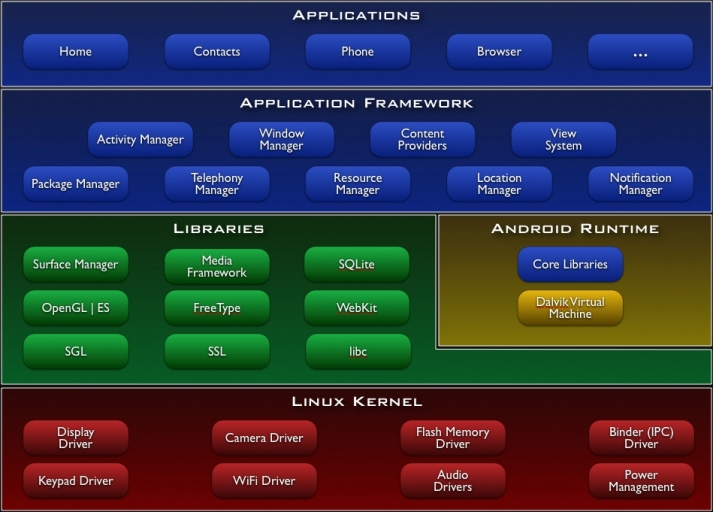
\includegraphics[width=0.9\textwidth]{android_system_architecture.jpg}
			\caption{Αρχιτεκτονική του λειτουργικού συστήματος Android}
			\label{fig:android_system_architecture}
		\end{figure}
		
		 Ξεκινώντας από το χαμηλότερο επίπεδο έχουμε \cite{collinsAndroid}\cite{annuzziAndroid}\cite{androidArchAnalysis}:
		 \begin{itemize}
		 	\item \textbf{Linux Kernel}: ο οποίος είναι ειδικά σχεδιασμένος για το λειτουργικό σύστημα Android και περιέχει τους οδηγούς για το υλικό (κάμερα, πληκτρολόγιο κ.τ.λ.). Επίσης ο πυρήνας είναι υπεύθυνος για τη διαχείριση της μνήμης και των διεργασιών, τις συνδέσεις δικτύου και κατ' επέκταση την διαχείριση των διεπαφών δικτύου που διαθέτει κάθε συσκευή. Επιπρόσθετα, χειρίζεται τους πόρους και την ενεργεία, κάτι το οποίο είναι πολύ σημαντικό δεδομένου της περιορισμένης παροχής ενέργειας των κινητών συσκευών. 
		 	\item \textbf{Libraries} Στο αμέσως επόμενο επίπεδο έχουμε τις βιβλιοθήκες του συστήματος, οι οποίες πολλές φορές αποκαλούνται και εγγενείς βιβλιοθήκες (Native Libraries). Οι εν λόγω βιβλιοθήκες έχουν αναπτυχθεί με χρήση των γλωσσών προγραμματισμού C και C++. Μερικές από τις πιο σημαντικές βιβλιοθήκες αυτού του επίπεδου είναι:
		 	\begin{itemize}
		 		\item WebKit, για την υποστήριξη των φυλλομετρητών
		 		\item Media Framework, για την αναπαραγωγή αρχείων ήχου και βίντεο
		 		\item Surface Manager, για τη δημιουργία παραθύρων και ανανέωση της οθόνης
		 		\item SQLite, για τη διαχείριση των βάσεων δεδομένων
		 		\item OpenGL, για την απόδοση γραφικών
		 		\item Text, για τον χειρισμό και την εμφάνιση κειμένου
		 	\end{itemize}
		 	Σε αυτό το επίπεδο βρίσκεται επίσης και το κομμάτι της εκτέλεσης του Android (Android Runtime), το οποίο υποστηρίζει τη διαδικασία εγγραφής και εκτέλεσης των εφαρμογών. Αποτελείται από δυο βασικές συνιστώσες:
		 	\begin{itemize}
		 		\item Βασικές βιβλιοθήκες για τη διεπαφή των εφαρμογών Java με το περιβάλλον της συσκευής στην οποία εκτελούνται. Πιο αναλυτικά, οι εν λόγω βιβλιοθήκες είναι δυναμικές, οι οποίες εισάγονται στην αρχή κάθε κλάσης.
		 		\item Την εικονική μηχανή Dalvik (Dalvik Virtual Machine) η οποία είναι υπεύθυνη για τη δημιουργία των εκτελέσιμων αρχείων των εφαρμογών. Συγκεκριμένα ο πηγαίος κώδικας Java μετατρέπεται σε μορφή ενδιάμεσου κώδικα (bytecode) και στην συνέχεια μεταφράζεται σε Dalvik bytecode που αποθηκεύεται σε αρχεία της μορφής .dex. Η διαδικασία της μετατροπής των αρχείων κλάσεων java σε μορφή .dex γίνεται από το εργαλείο dx, ενώ παράλληλα γίνεται και βελτιστοποίηση της πλεονάζουσας πληροφορίας με αποτέλεσμα τα αρχεία .dex να είναι μικρότερα σε μέγεθος από τα αντίστοιχα αρχεία κλάσεων. Τέλος, το αρχείο .dex μαζί με τους πόρους της εφαρμογής μετατρέπονται σε αρχείο της μορφή .apk (Android Package). Το .apk αρχείο είναι αυτό που χρησιμοποιείται από τον χρήστη για την εγκατάσταση της εφαρμογής στην συσκευή του. Όταν ο χρήστης εκτελέσει την εφαρμογή, τότε η εφαρμογή αυτή θα εκτελεστεί στην εικονική μηχανή Dalvik αντί της JVM, καθώς το περιβάλλον εκτέλεσης των κινητών συσκευών διαθέτει περιορισμένους πόρους.
		 	\end{itemize}
		 	\item \textbf{Application Framework} Στο τρίτο επίπεδο βρίσκεται το πλαίσιο λογισμικού των εφαρμογών, το οποίο ουσιαστικά είναι ένα σύνολο υπηρεσιών, οι οποίες δημιουργούν το περιβάλλον μέσα στο οποίο εκτελούνται οι εφαρμογές Android. Μερικές από τις πιο βασικές υπηρεσίες που περιλαμβάνονται στο επίπεδο του applicaiton framework είναι οι παρακάτω:
		 	\begin{itemize}
		 		\item Package Manager: Ο διαχειριστής πακέτων είναι το σύστημα μέσω του οποίου οι εφαρμογές μπορούν να βρουν πληροφορίες για τις υπόλοιπες εφαρμογές που είναι εγκατεστημένες στη συσκευή. Αποτελεί ουσιαστικά μια βάση δεδομένων όλων των εφαρμογών που είναι εγκατεστημένες στην συσκευή και επιτρέπει σε μια μια εφαρμογή να χρησιμοποιήσει μια άλλη και να μοιραστεί δεδομένα με αυτήν.
		 		\item Activity Manager: Ο διαχειριστής δραστηριοτήτων διαχειρίζεται τον κύκλο ζωής των εφαρμογών και τη στοίβα δραστηριοτήτων (activity stack).
		 		\item Content Providers: Οι πάροχοι περιεχομένου επιτρέπουν στις εφαρμογές να δημοσιεύουν και να μοιράζονται δεδομένα με άλλες εφαρμογές. Αποτελούν ουσιαστικά βάσεις δεδομένων οι οποίες δίνουν την δυνατότητα στις εφαρμογές να αποθηκεύσουν και να μοιραστούν δομημένες πληροφορίες. Παράδειγμα τέτοιων πληροφοριών αποτελούν οι επαφές της συσκευής.
		 		\item View System: Περιλαμβάνει γραφικά στοιχεία τα οποία χρησιμοποιούνται για τη δημιουργία της διεπαφής χρήστη. Παράδειγμα γραφικών στοιχείων που περιλαμβάνει είναι κουμπιά, κουτιά κειμένων, πλαίσια κ.τ.λ.
		 		\item Resource Manager: Ο διαχειριστής πόρων είναι υπεύθυνος για τη διαχείριση των πόρων που δεν αποτελούν κώδικα και κατ' επέκταση δεν μπορούν να μεταγλωττιστούν. Παράδειγμα τέτοιων στοιχείων αποτελούν τα γραφικά στοιχεία και οι συμβολοσειρές.
		 		\item Notification Manager: Ο διαχειριστής ειδοποιήσεων επιτρέπει στις εφαρμογές να εμφανίζουν ειδοποιήσεις προς το χρήστη. Οι ειδοποιήσεις αυτές εμφανίζονται στη μπάρα κατάστασης της συσκευής, η οποία βρίσκεται στο πάνω μέρος της οθόνης και είναι σχεδόν πάντα ορατή στον χρήστη.
		 		\item Telephony Manager: Ο διαχειριστής τηλεφωνίας παρέχει πληροφορίες στην εφαρμογή σχετικά με τις υπηρεσίες τηλεφώνου που είναι διαθέσιμες στην συσκευή.
		 		\item Location Manager: Ο διαχειριστής τοποθεσίας παρέχει στις εφαρμογές πρόσβαση σε πληροφορίες σχετικά με την τοποθεσία και την κίνηση της συσκευής.
		 	\end{itemize}
		 	\item \textbf{Applications} Στο τέταρτο και τελευταίο επίπεδο της αρχιτεκτονικής του λειτουργικού συστήματος Android βρίσκονται οι εφαρμογές. Σε αυτό το επίπεδο περιλαμβάνονται τόσο οι προεγκατεστημένες εφαρμογές όσο και οι εφαρμογές τρίτων.
		 \end{itemize}
		 
		\subsubsection{Δομικά στοιχεία του Android}
		Υπάρχουν τέσσερα βασικά δομικά στοιχεία στο λειτουργικό σύστημα Android (βλ. σχήμα \ref{fig:android_fundamental_components}). Κάθε δομικό στοιχείο επιτελεί ένα ξεχωριστό σκοπό και έχει ανεξάρτητο κύκλο ζωής. Κάθε δομικό στοιχείο αποτελεί ουσιαστικά ένα διαφορετικό σημείο, μέσω του οποίου το λειτουργικό σύστημα μπορεί να αποκτήσει πρόσβαση στην εφαρμογή. Στην συνέχεια θα κάνουμε μια συνοπτική παρουσίαση των βασικών αυτών δομικών στοιχειών, θεμελιώνοντας έτσι το θεωρητικό πλαίσιο για ανάπτυξη εφαρμογών Android \cite{androidComponentsKnoxville}\cite{androidFundamentalsOfficial}.
		
		\begin{figure}[h]
			\centering
			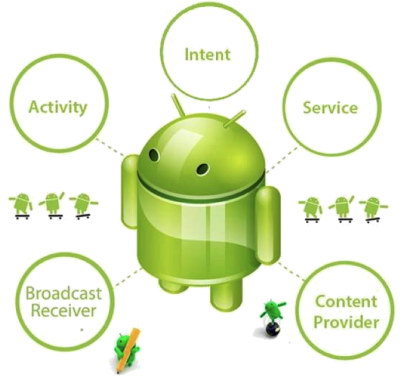
\includegraphics[width=0.6\textwidth]{android_fundamental_components.jpg}
			\caption{Δομικά στοιχεία του Android.}
			\label{fig:android_fundamental_components}
		\end{figure}
		
		\subsubsection{Activities}
		Η κλάση Activity αποτελεί τη βασικότερη κλάση μιας εφαρμογής Android. Κάθε κλάση Activity αποτελεί μια ξεχωριστή γραφική διεπιφάνεια (παράθυρο/οθόνη) μέσω της οποίας ο χρήστης αλληλεπιδρά με την εφαρμογή. Συνήθως το παράθυρο αυτό καλύπτει όλη την οθόνη της συσκευής αλλά υπάρχουν και κάποιες εξεζητημένες περιπτώσεις στις οποίες καλύπτει μόνο ένα μέρος της οθόνης.
		
		Κάθε εφαρμογή αποτελείται κατά κανόνα από πολλές Activities (οθόνες), οι οποίες είναι συνδεδεμένες μεταξύ τους, ενώ έχουν και την δυνατότητα ανταλλαγής πληροφοριών. Η οθόνη που παρουσιάζεται πρώτη στον χρήστη με το που πραγματοποιήσει εκκίνηση της εφαρμογής ονομάζεται `κύρια' (main), μέσω της οποίας μπορεί να πλοηγηθεί και στις υπόλοιπες οθόνες. Εν γένει κάθε activity έχει τη δυνατότητα να πραγματοποιήσει εκκίνηση μια άλλης activity. Το σύστημα κάθε φορά που γίνεται μετάβαση σε μια νέα activity εισχωρεί (push) την προηγούμενη σε μια στοίβα μορφής LIFO, που ονομάζεται back-stack, έτσι ώστε αν ο χρήστης πατήσει το κουμπί επιστροφής (back) να μπορεί με ένα pop στην στοίβα να επαναφέρει την αμέσως προηγούμενη activity. Δηλαδή αν ήμασταν αρχικά στην activity Α μέσω της οποία μεταβήκαμε στην Β, η activity Α βρίσκεται στην κορυφή της στοίβας οπότε με το πλήκτρο back οδηγούμαστε πάλι στην οθόνη που βρισκόμασταν προηγουμένως την Α. Σε αυτό το σημείο θα πρέπει να αναφερθεί ότι αν πατηθεί το κουμπί back όταν ο χρήστης βρίσκεται στην αρχική οθόνη και η στοίβα είναι άδεια, πραγματοποιείται έξοδος από την εφαρμογή.
		
		Για τη δημιουργία μιας οθόνης θα πρέπει να κάνουμε extend τη βασική κλάση Activity και να υλοποιήσουμε κάποιες απαραίτητες μεθόδους της. Συγκεκριμένα κάθε activity  πρέπει να υλοποιεί τη μέθοδο onCreate(), η οποία καλείται αυτόματα κατά την πρώτη εκκίνηση της activity όπως υπονοεί και το όνομα της. Θα πρέπει να τονιστεί ότι εκτελείται μόνο κατά την πρώτη δημιουργία του activity και όχι όταν επιστρέφουμε σε αυτό με χρήση του κουμπιού της επιστροφής. Μέσα στην εν λόγω μέθοδο γίνεται αρχικοποίηση των βασικών συστατικών που αποτελούν τη διεπαφή του χρήστη.
		
		Μια επίσης εκ των βασικών μεθόδων που πρέπει να υλοποιήσουμε αποτελεί το onPause(). Όπως υποδηλώνει και το όνομά της καλείται από το σύστημα όταν ο χρήστης πραγματοποιεί έξοδο από το συγκεκριμένο activity χωρίς όμως να το καταστρέφει, για παράδειγμα όταν κάνει μετάβαση σε άλλο activity της ίδιας εφαρμογής.
		
		Για να πραγματοποιήσουμε τον τερματισμό ενός activity αρκεί να εκτελεστεί η εντολή finish(), αν και συνήθως δεν χρειάζεται να τερματίζουμε εμείς τις acitivities αφού είναι κάτι που αποτελεί ουσιαστικά δικαιοδοσία του Dalvik. Για να γίνουν καλύτερα κατανοητά τα παραπάνω στο σχήμα \ref{fig:activity_lifecycle} βλέπουμε τον κύκλο ζωής των activities και τις αντίστοιχες μεθόδους.
		
		\begin{figure}[h]
			\centering
			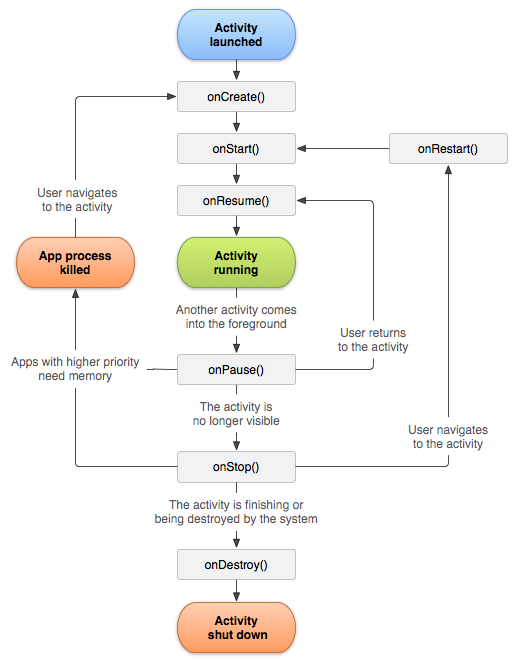
\includegraphics[width=0.5\textwidth]{activity_lifecycle.png}
			\caption{Ο κύκλος ζωής των activities.}
			\label{fig:activity_lifecycle}
		\end{figure}
		
		\subsubsection{Services}
		Οι υπηρεσίες αποτελούν τα στοιχεία μιας εφαρμογής, οι οποίες εκτελούν χρονοβόρες λειτουργίες στο παρασκήνιο (background) της εφαρμογής. Θεμελιώδη διαφορά μεταξύ μιας υπηρεσίας και ενός activity αποτελεί το γεγονός ότι η υπηρεσία δεν παρέχει κάποια διεπαφή προς τον χρήστη της εφαρμογής, δεδομένου ότι όπως προαναφέρθηκε δρουν παρασκηνιακά. Μια υπηρεσία έχει την δυνατότητα να συνεχίζει την εκτέλεση της στο παρασκήνιο ακόμα και στην περίπτωση όπου ο χρήστης έχει πραγματοποιήσει μετάβαση σε κάποια τελείως διαφορετική εφαρμογή. Ένα κλασσικό παράδειγμα υπηρεσίας αποτελεί η αναπαραγωγή μουσικής, η οποία συνεχίζει να εκτελείται στο παρασκήνιο ακόμα και όταν έχουμε κλείσει την εφαρμογή αναπαραγωγής μουσικής και εκτελούμε τελείως διαφορετικές εφαρμογές. Υπάρχουν κάποιες έτοιμες υπηρεσίες που μας παρέχει το λειτουργικό σύστημα όπως είναι ο Location Manager, αλλά μπορούμε να ορίσουμε και τις δικές μας υπηρεσίες. Μια υπηρεσία μπορεί ουσιαστικά να πάρει δυο διαφορετικές μορφές\cite{servicesAndroid}:
		\begin{itemize}
			\item Started: Μια υπηρεσία έχει εκκινηθεί όταν κάποιο συστατικό της εφαρμογής (π.χ ένα activity) έχει καλέσει τη μέθοδο startService(). Μόλις η υπηρεσία εκκινηθεί συνεχίζει να εκτελείται επ' αόριστον στο παρασκήνιο ακόμα και αν το activity που τηn κάλεσε έχει τερματιστεί. Συνήθως επιτελεί μία και μόνο εργασία χωρίς να επιστρέφει κάποιο αποτέλεσμα στο activity που την κάλεσε. Για παράδειγμα, μπορεί να κατεβάζει κάποιο αρχείο και όταν ολοκληρωθεί η μεταφόρτωση του θα τερματίσει η ίδια τον εαυτό της.
			\item Bound: Λέμε ότι μια υπηρεσία είναι ``δεμένη'' όταν κάποιο συστατικό της εφαρμογής (π.χ ένα activity) έχει καλέσει την μέθοδο bindService(). Μια `δεμένη' υπηρεσία παρέχει διεπαφή πελάτη - εξυπηρετητή (client - server) και επιτρέπει στα συστατικά της εφαρμογής που είναι συνδεδεμένα μαζί της να αλληλεπιδρούν με αυτήν, στέλνοντας αιτήματα και λαμβάνοντας τα αποτελέσματα ακόμα και αν βρίσκονται σε διαφορετικές διεργασίες χρησιμοποιώντας IPC (interprocess communication). Υπηρεσίες τέτοιου τύπου συνεχίζουν τη λειτουργία τους όσο τα συστατικά με τα οποία είναι συνδεδεμένα εξακολουθούν να τρέχουν. Η υπηρεσία τερματίζεται μόνο όταν τερματιστεί (ή αποσυνδεθεί) και το τελευταίο συστατικό που είναι συνδεδεμένο με αυτήν.
		\end{itemize}
		Όπως αναφέρθηκε προηγουμένως οι υπηρεσίες δεν παρέχουν κάποια διεπαφή προς τον χρήστη, οπότε δημιουργείται και το εύλογο ερώτημα για το πως θα ενημερώνεται ο χρήστης. Οι υπηρεσίες ειδοποιούν τους χρήστες για τα αποτελέσματα τους είτε με χρήση ειδοποίησης μορφής Toast είτε μέσω ειδοποίησης στο status bar.  Για να γίνουν καλύτερα κατανοητά οι έννοιες που αναλύθηκαν παραπάνω στο σχήμα \ref{fig:service_lifecycle} βλέπουμε τον κύκλο ζωής των υπηρεσιών.
		
		\begin{figure}[h]
			\centering
			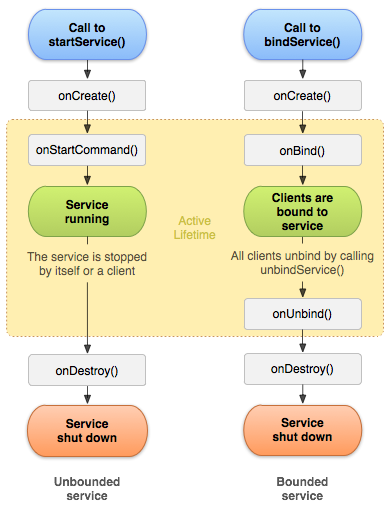
\includegraphics[width=0.5\textwidth]{service_lifecycle.png}
			\caption{Ο κύκλος ζωής των services}
			\label{fig:service_lifecycle}
		\end{figure}
		
		\subsubsection{Content Providers}
		Οι πάροχοι περιεχομένου διαχειρίζονται την πρόσβαση στους αποθηκευτικούς χώρους των δεδομένων. Ουσιαστικά, δημιουργείται η δυνατότητα αποθήκευσης και διαμοιρασμού δεδομένων στις εφαρμογές. Ένας πάροχος δεδομένων παρουσιάζει τα δεδομένα στις εφαρμογές σε μορφή πινάκων σαν τους πίνακες σε μια σχεσιακή βάση δεδομένων. Παράδειγμα ενός ενσωματωμένου παροχέα δεδομένων είναι το λεξικό χρήστη στο οποίο αποθηκεύονται οι λέξεις του χρήστη. Για αυτή τη χρήση υπάρχει και η ενσωματωμένη βάση δεδομένων SQLite, η οποία δίνει την δυνατότητα αποθηκεύσης και ανάγνωσης δεδομένων στους παρόχους περιεχομένου.\cite{androidContentProviders}
		\subsubsection{Broadcast Receivers}
		Οι δέκτες εκπεμπόμενων προθέσεων είναι υπεύθυνοι για τη λήψη και τη διαχείριση των γεγονότων που πραγματοποιούνται στην συσκευή. Συγκεκριμένα, ενημερώνονται από το λειτουργικό σύστημα όταν πραγματοποιείται κάποιο γεγονός και τότε ενεργοποιούνται. Χαρακτηριστικά παραδείγματα τέτοιων γεγονότων είναι όταν το κινητό μπαίνει σε κατάσταση αναμονής, όταν η στάθμη της μπαταρίας είναι χαμηλή κ.τ.λ. Οι δέκτες εκπεμπόμενων προθέσεων δεν παρέχουν κάποια διεπαφή προς τον χρήστη όπως και οι υπηρεσίες και μπορούν να επικοινωνήσουν με τον χρήστη μέσω ειδοποιήσεων στο status bar.\cite{broadcastReceiver}

%		\textbf{Material design ? Αν δεν είναι API Level 21?}
%	\subsection{Mockups}
%	\subsection{Διασύνδεση με Social Networks}
%	Όπως παρουσιάσαμε και στο την ενότητα  \ref{ssec:social_netowrks_system_analysis} η διασύνδεση με τα μέσα κοινωνικής δικτύωσης αποτελεί θέμα μείζονος σημασίας για την εφαρμογή έξυπνου κινητού του συστήματος μας, καθώς παίζει καθοριστικό ρόλο στην επίτευξη των στόχων που θέσαμε στην ενότητα \ref{sec:intro_goals}. Δηλαδή στην προσέλκυση νέων εθελοντών αιμοδοτών αλλά και στην διατήρηση (retention) των υπαρχόντων εθελοντών. Στο παρόν κεφάλαιο θα γίνει μια σύντομη αναφορά στον τρόπο διασύνδεσης μιας εφαρμογής android με το κοινωνικό δίκτυο facebook.
%	
%%		\subsubsection{Facebook Integration}
%%		Το facebook παρέχει προς τους προγραμματιστές SDKs - Software Development Kits (Κιτ ανάπτυξης λογισμικού), μέσω του οποίου μπορούν να πραγματοποιήσουν εύκολη επικοινωνία μεταξύ της εφαρμογής που αναπτύσσουν και των υπηρεσιών που παρέχει το Facebook. Συγκεκριμένα μέσω του Android SDK που χρησιμοποιήθηκε στα πλαίσια της παρούσας διπλωματικής εργασίας, δίνεται η δυνατότητα να χρησιμοποιηθούν οι παρακάτω υπηρεσίες του facebook\cite{facebookApiCapabilities}:
%%		\begin{itemize}
%%			\item Facebook Login: Σύνδεση με χρήση του λογαριασμού που ο χρήστης διατηρεί στο facebook
%%			\item Share and send dialogs: Διαμοιρασμός περιεχομένου της εφαρμογής στο facebook
%%			\item App events: Καταγραφή της συμπεριφοράς του χρήστη
%%			\item Graph API: Δυνατότητα γραφής και ανάγνωσης στο Graph API
%%		\end{itemize}
%%		
%%	Το πρώτο βήμα για την διασύνδεση μεταξύ εφαρμογής έξυπνου κινητού και facebook είναι η δημιουργία μίας εφαρμογής στο Facebook. Κατά την δημιουργία της εφαρμογής θα πρέπει να εισαχθούν κάποια διαπιστευτήρια της εφαρμογής έξυπνου κινητού όπως το Google Play package name αλλά και το hask key της εφαρμογής.
%%	
%		Στη συνέχεια θα κάνουμε μια σύντομη ανάλυση για τις υπηρεσίες διαμοιρασμού περιεχομένου και επικοινωνίας με το Graph API, τις οποίες και χρησιμοποιήσαμε κατά την ανάπτυξη του συστήματος της παρούσας διπλωματικής.
